%!TEX encoding = UTF-8 Unicode
\documentclass[12pt]{article} 
\usepackage{tikz}

%\usepackage{xcolor}
%\usepackage{hyperref}
%\usepackage{subfig}
%\usepackage{xltxtra} 
\usepackage{enumerate}
\usepackage{amsmath,amsthm,amssymb,amsfonts} 
\usepackage{graphicx} 
\usepackage[center]{caption} 
\usepackage{enumerate} 
\usepackage[shortlabels]{enumitem} 
\setlength{\marginparwidth}{2cm}
\usepackage[obeyDraft,colorinlistoftodos]{todonotes} 
\usepackage[onehalfspacing]{setspace}

\usepackage{array}

%\usepackage{fontspec}
%\usepackage{xunicode}
%\usepackage{xltxtra} \synctex=1 
\usepackage[longnamesfirst]{natbib}
\usepackage{subcaption} 
\usepackage[onehalfspacing]{setspace}

\usepackage{soul}

%\usepackage[round]{natbib}
%\usepackage[all]{xy}
%\setcounter{MaxMatrixCols}{10}
%
\renewcommand{\l}{\ell}
\newtheorem{theorem}{Theorem}
\newtheorem{acknowledgement}{Acknowledgement}
\newtheorem{algorithm}{Algorithm}
\newtheorem{assumption}{Assumption}
\newtheorem{axiom}{Axiom}
\newtheorem{case}{Case}
\newtheorem{claim}{Claim}
\newtheorem{conclusion}{Conclusion}
\newtheorem{condition}{Condition}
\newtheorem{conjecture}{Conjecture}
\newtheorem{corollary}{Corollary}
\newtheorem{criterion}{Criterion}
\newtheorem{example}{Example}
\newtheorem{exercise}{Exercise}
\newtheorem{lemma}{Lemma}
\newtheorem{proposition}{Proposition} \theoremstyle{definition}
\newtheorem{definition}{Definition}
\newtheorem{notation}{Notation}
\newtheorem{problem}{Problem} \theoremstyle{remark}
\newtheorem{remark}{Remark}
\newtheorem{fact}{Fact}
\newtheorem{solution}{Solution}
\newtheorem{summary}{Summary}

\newtheoremstyle{break}
  {\topsep}{\topsep}%
  {\itshape}{}%
  {\bfseries}{}%
  {\newline}{}%
\theoremstyle{break}

\newtheorem{thm}{Theorem}[subsection]
\newtheorem{lem}[thm]{Lemma}
\newtheorem{prop}[thm]{Proposition}\theoremstyle{break}
\newtheorem{cor}[thm]{Corollary} 
\newtheorem{result}{Experimental Result}\theoremstyle{break}


\begin{document}
\title{Cheap Talk is not Cheap: Free versus Costly Communication\footnote{%
For valuable comments and discussion, the authors are grateful to Vincent Crawford and conference and seminar participants at ThRed 2017, University of Essex, Royal Economic Society, Universit\'e libre de Bruxelles and Groningen. Legros gratefully acknowledges the financial support of the European Research Council under the European Union's Seventh Framework Programme (FP7/2007-2013) / ERC grant agreement n$^0$ 339950. Hamid Aghadadashli was a postdoc at ECARES during the completion of this project.} }
\author{ 
\begin{tabular}{ccc}
Hamid Aghadadashli\footnote{Universit\'e libre de Bruxelles (ECARES). Present address: NERA Economic Consulting.}&  Georg Kirchsteiger\footnote{Universit\'e libre de Bruxelles (ECARES), CESifo and CEPR.} & Patrick Legros\footnote{Universit\'e libre de Bruxelles (ECARES), Northeastern University and CEPR.}
\end{tabular}
}
\date{This version: \today}
\maketitle
\newpage
\begin{abstract}
\singlespacing
The paper studies the effectiveness of communication in a two-player two-sided asymmetric information context. Both players choose simultaneously between two actions, with action $L$ leading to a lower payoff for the co-player than action $H$. There are two types of players: $D$-types for whom $L$ is dominant, and $C$-types for whom the optimal action is the same as the one chosen by the co-player, with both player choosing $H$ providing the $C$-type a higher payoff than both players choosing $L$. Before the actions are chosen, each player can signal his/her intention to choose $H$. We consider three communication environments: No communication (NC), cheap talk (CT), and an environment with extrinsic communication costs (FC). For this game the range of equilibrium payoffs of both types is the same in NC and CT, while for $C$-types the equilibrium payoff is highest in FC due to the Spence mechanism (Spence 1973). When we tested these predictions experimentally, the $C$-type payoffs were the highest in CT. In this environment the average observed $C$-type payoff was even higher than the maximum equilibrium payoff. In CT about half of the $D$-types did not mimic the communication behavior of $C$-types, and hence even cheap talk revealed some information to the $C$-types. This indicates that half of the $D$-types were reluctant to make promises they would break. We introduce a theoretical model with promise-keepers. When the probability of an agent being promise-keeper is around 50\%, the signaling rate will be higher in CT than in FC. On the other hand, for the same signal structure $C$-types choose more often $H$ in the FC than in CT. These predictions are confirmed by the experimental results. Overall, the effect of the higher signalling rate in CT dominates: Together with presence of promise-keepers the higher signalling rate allows the $C$-types to coordinate more often on the ``good'' $(H,H)$ outcome in CT, resulting in higher $C$-type payoffs in CT than in FC.
\end{abstract}
\noindent\textit{Keywords:} credible communication, asymmetric information, coordination\\
\noindent\textit{JEL classification:} C7, C9.

\pagebreak
\section{Introduction}
Communication is one of the defining aspects of human interaction. But whenever communicating agents have conflicts of interest, the ability of communicating private information becomes an issue. Starting with the seminal contribution of \cite{Spence1973}, the research on signalling games has shown that costs of communication are crucial for the credibility of communication. While in general cheap talk can impact the set of equilibrium payoff vectors (see e.g. the classical paper of \cite{Crawford1982} in the context of one-sided incomplete information), costless communication does not make any difference in many economically important contexts. On the other hand, costly communication can make communication credible, depending on the available actions and on the payoff structure. In such situations communication costs should never hinder credible communication, and for many economically important situations it should actually enhance the possibilities of credible communication (compared to pure cheap talk).

This paper tests this prediction experimentally in the context of two-sided asymmetric information. On top of the economic relevance of two-sided asymmetric information, we use a two-sided asymmetric information structure in order to distinguish between the impact of one-sided and two-sided signals. Two players have to choose simultaneously between two actions with one action (action ``$L$") leading to a lower payoff for the co-player than the other action (action ``$H$"). Concerning the own payoff, there are two types of players: $D$-types for whom $L$ is dominant, and $C$-types who want to play $H$ if the co-player does the same. If the co-player plays $L$, a $C$-type's optimal action is also $L$. Hence, a pair of $C$-types would play a coordination game if the types were common knowledge. Furthermore, coordination on $(H,H)$ is better for $C$-types than coordination on $(L,L)$. Because of this payoff structure, knowledge about the type of the co-player is crucial for $C$-types (but not for $D$-types): If both players are $C$-types, and this is common knowledge, coordination on $(H,H)$ is the payoff- and risk-dominant equilibrium. But if the co-player is a $D$-type, for whom the choice of $H$ is strictly dominated, a $C$-type would choose $L$.

If communication is possible, each player decides whether to send a signal to his/her co-player that (s)he will play $H$. Both players decide simultaneously about the signal. After being informed about the signals, both players decide simultaneously which action to choose.

We consider three communication environments: No communication (NC); cheap talk (CT), where each player can signal his intention to choose $H$ to her/his co-player without any costs; and an environment with communication costs (FC), where each player has the costly opportunity to inform her/his co-player about her/his intention to play $H$.

We show that the introduction of cheap talk communication should not make a difference - the range of equilibrium payoffs of both types is the same in NC and in CT. On the other hand, the maximum equilibrium payoff of the $C$-types is higher in FC due to the Spence mechanism. To our surprise, these predictions were not confirmed by the experimental results. The observed payoffs of the $C$-types were much larger in CT than in the other environments, in fact the observed CT-payoffs of $C$-types were even larger than the highest payoffs predicted by any equilibrium of the standard model.

Closer inspection of the communication behavior reveals that contrary to the theoretical predictions about half of the $D$-types did not mimic the communication behavior of the $C$-types. They did not promise to play $H$ despite having a monetary incentive to do so. This makes the signal informative for $C$-types, which in turn allows pairs of $C$-types to coordinate on the ``good'' action combination $(H,H)$. To check whether this reluctance to make wrong promises can indeed explain the experimental results, we introduce a model where each player has a 50\% chance of being a promise-keeper, i.e. a player who keeps his promises whenever (s)he makes such a promise, and a 50\% chance of being a standard opportunistic player. Whether a player is a promise-keeper or not is private information of this player\footnote{%
Since the interaction is one-shot, there is no possibility that players could signal whether they are promise-keepers or opportunists.}, and it is independent of whether the player is a $D$- or a $C$-type.

Using this framework and the payoffs used in the experiment, the theoretical results suggest that the signaling rate will be higher in CT than in FC. In both environments, the probability of $C$-types choosing $H$ increases in the amount of signalling. This would imply that we should observe more $H$-choices in CT than in FC. But on the other hand, for the same signal structure $C$-types are more likely to choose $H$ in FC than in CT. In particular, a $C$-type is more likely to choose $H$ in FC than in CT when the co-player does not signal. Overall, the effect of the higher signalling rates in CT dominates: When two $C$-types are are matched in CT, both send a signal and both play $H$ for sure, leading to perfect coordination on the good outcome $(H,H)$. In FC, only a fraction of $C$-types sends the signal, and therefore a $(C/C)$-pair does not for sure coordinate on $(H,H)$. This in turn leads to lower payoffs for the $C$-types in FC than in CT. 

The experimental results confirm these theoretical predictions. While in CT nearly all cooperators and about half of the defectors signal their willingness to cooperate, only about half of the $C$-types and hardly any of the $D$-types communicate in FC. We also find that for given communication outcome the $C$-types are more likely to play $H$ in FC than in the CT. This is in particular true when only one player sends a signal. As predicted the first effect dominates - $(C/C)$-pairs coordinate considerably more often on $(H,H)$ in CT than in FC.

 \subsection*{Related Literature}
The classical paper by \cite{Spence1973} illustrates how costs of communication can facilitate credible communication of private information. In Spence's model with one-sided asymmetric information, one has to distinguish between the sender who has private information and can send a signal, and the receiver who wants to know the private information of the sender and receives the sender's signal. In this framework different types of senders have similar preference-orders on outcomes. It is therefore important that different types of senders have different costs of communication for the receiver to be able to sort out types in equilibrium. In our context of a game with two-sided private information, both players are senders and receivers at the same time, and different types of players have different preference-orders on outcomes. Hence, even if both types of players face the same costs of communication, different types have have different incentives to use communication.

%While sorting is facilitated with an exogenous cost, it is not always the case that the payoffs net of the cost of communication of the ``good'' types are larger with costly communication than without costly communication.\footnote{%Indeed, in a sorting equilibrium, the cost of deviating and not communicating leads to the lowest productivity wage, while in the non-informative equilibrium all types get the expected productivity wage. For stability we need $yH-cH>yL$ and $y_L>yH-cL$ but this may be consistent with $yH-cH < E[y]$.}

The fact that costless signals may lead to informative communication has received ample experimental support, see the survey by \cite{crawford1998} on ``cheap talk'' experiments and why the results contradict the theoretical view that cheap talk should not matter. Recently, \cite{abeler2019} review 72 experiments in the tradition of \cite{fischbacher2013} where agents get information and receive a payment proportional to their report. \cite{abeler2019} conclude that these experimental results are  best explained when individuals are assumed to have both a ``preference for being honest and a preference for being seen as honest.'' 

In the context of a principal-agent experiment \cite{charness2006} argue that agents tend to keep their promises in order to avoid guilt. A follow-up paper by \cite{charness2011} analyzes the role that costless communication plays in a one-sided hidden information setting. \cite{jacquemet2018} show that allowing agents to sign an ``oath not to lie'' before playing a game increases communication and coordination. In the context of sender receiver games with one-sided asymmetric information, \cite{cai2006} and \cite{Wang2010} report excessive truth-telling compared to the theoretical analysis of \cite{Crawford1982}. \cite{Wang2010} and \cite{Crawford2013} explain this excessive truth-telling by level-k thinking.  




%Oath literature: see for instance \cite{jacquemet2018} where players can sign an oath not to lie before a cheap talk game before playing a coordination game with perfect information. Signing the form is not observed by other participants.  

All this literature is either limited to perfect information, or to one-sided imperfect information settings. Furthermore, it does not consider the possibility of having both extrinsic communication costs and an intrinsic motivation to tell the truth. To our knowledge our paper is the first investigating the interplay between extrinsic communication costs and an intrinsic unwillingness to lie and to break promises.

%On top of collusion, there are many other situations characterized by two-sided experimental analysis (examples). However, most of the existing literature focuses on one-sided asymmetric information. The experimental signalling games dealt mainly with testing equilibrium refinements like the Cho-Kreps criterion (see e.g. Brandts and Holt 1992 AER) and learning behavior in these games (see e.g. Cooper et al 1997 Rand)

The rest of the paper is structured as follows: In the next section we present the experimental game with two-sided asymmetric information. In section 3 we describe the experimental design. In section 4 we contrast the predictions of the standard model and the experimental results. In section 5 we extend the standard model to allow for promise-keeping behavior, and show that the predictions of this extended model fits the experimental data. We offer some final comments in the last section.

\section{The Experimental Game}

There were two players playing a two-sided asymmetric information game with two stages. Each player was either of type $C$ or of type $D$ with an equal probability of $1/2$. The type of a player was private information - it was only revealed to the player him/herself, but not to the co-player. In the first stage of the game, the players had the opportunity to send each other signals (``communication stage"). In the second stage of the game, both players chose simultaneously an action from the action set $\{H,L\}$. A player's payoff depended on his/her own type and on the actions of both players. The payoff matrices were as follows:
	\begin{table}[!htbp]
    	\centering
		\begin{tabular}{c c c}
			  & H   & L   \\ \cline{2-3}
			H & \multicolumn{1}{|c|}{$50$, $50$} & \multicolumn{1}{c|}{$10$, $24$} \\ \cline{2-3}
			L & \multicolumn{1}{|c|}{$24$, $10$} & \multicolumn{1}{c|}{$20$, $20$} \\ \cline{2-3}
            \\
            \multicolumn{3}{c}{Type $C$ vs Type $C$} \\
		\end{tabular}
		\hfill
   		\begin{tabular}{c c c}
			  & H   & L   \\ \cline{2-3}
			H & \multicolumn{1}{|c|}{$50$, $22$} & \multicolumn{1}{c|}{$10$, $24$} \\ \cline{2-3}
			L & \multicolumn{1}{|c|}{$24$, $10$} & \multicolumn{1}{c|}{$20$, $20$} \\ \cline{2-3}
			\\
            \multicolumn{3}{c}{Type $C$  vs Type $D$} \\
		\end{tabular}
        \hfill
   		\begin{tabular}{c c c}
			  & H   & L   \\ \cline{2-3}
			H & \multicolumn{1}{|c|}{$22$, $22$} & \multicolumn{1}{c|}{$10$, $24$} \\ \cline{2-3}
			L & \multicolumn{1}{|c|}{$24$, $10$} & \multicolumn{1}{c|}{$20$, $20$} \\ \cline{2-3}
			\\
            \multicolumn{3}{c}{Type $D$ vs Type $D$} \\
		\end{tabular}
        \caption{Payoffs depending on the actions chosen and on the type of the players - first player choosing the row.}\label{game_table}
	\end{table}
\newline
%
Before the players chose their actions, they had the opportunity to communicate with each other about their intended second stage choice. More specifically, both players chose simultaneously between sending the promise ``I will play $H$'' to the co-player or sending no signal at all. Crucially, the promise was not binding - a player was allowed to promise ``I will play $H$'' and then choose $L$ without any negative payoff consequences for the ``promise-breaker". 
We used three different communication environments: In the first environment, making the promise was connected to a fee of 3 (``communication fee environment'' FC). These communication costs were subtracted from the payoff the communicating player earned in the second stage as depicted in the table above. 
In the second environment sending the signal was not connected to any costs (``cheap talk environment'' CT).
As a benchmark, we also introduced a third environment where players could not communicate at all (``no communication'' environment NC). In this environment players could only choose their second stage actions.

\section{The Experimental Design}

In each experimental session one of the three communication environments was implemented. There were three sessions per environment. 72 subjects participated in CT and FC. Due to no show-ups, only 56 subjects participated in the NC. Each subject participated in only one experimental session, and overall 200 subjects participated in the experiment.
Each subject played the game 15 times, i.e., each session lasted for 15 rounds. At the beginning of each round, the type of each subject was determined randomly and independently with equal probability for each type. Subjects got re-matched every round according to a pre-defined matching protocol (strangers' treatment). Subjects were not informed about the identities of their co-players, but they knew that they were re-matched every round. 

Unknown to the subjects, the matching protocol was such that in each session there were three subgroups. Subjects were only matched with other members of their own subgroup. This matching protocol allows for three independent observations per session, and hence for 9 independent observations per treatment. 

The parameters of the earning functions were as described in the previous section. These earnings were in Experimental Currency Units (ECU). All the earnings a subject made in all the rounds were added up, and the sum was exchanged from ECUs into Euros. The exchange rate between Euros and ECUs was 1:25. In addition to the earning from the experimental game, all the subjects were given 4 Euros show-up fee. This resulted in an average payment of 18.18 Euros per subject. The average duration of a session was 70 minutes. The experiment took place at the DICE Lab at the University of D\"{u}sseldorf, Germany, using the software z-Tree \citep{fischbacher2007}. The instructions were in German. The translation of the instructions into English can be found in Appendix C. The German instructions are available from the authors upon request.

\section{Testing the Standard Model}\label{sec:standard-setting}

Like in the game with complete information, playing $H$ is strictly dominated by playing $L$ for the $D$-types when the types are private information. This is true for all communication environments. For $C$-types, the situation is more complicated. They want to play $H$ provided that the likelihood of the co-player also choosing $H$ is large enough. But they do not know the type of the co-player. In NC, where communication is not possible, $C$-type players face a coordination problem with other $C$-type players. Denote by $x$ the likelihood that a $C$-type plays $H$ in NC. The set of Nash equilibria is given by: (all proofs are relegated to the Appendix A)
%
\begin{proposition}\label{prop:NC} NC exhibits three Nash equilibria:
	\begin{enumerate}[i)]\setlength\itemsep{0em}
		\item $x = 1$, and the $D$-types choose $L$. The expected equilibrium payoffs are $30$ for the $C$-type players and $22$ for the $D$-type players.
		\item $x = 0$, and the $D$-types choose $L$. The expected equilibrium payoffs are $20$ for both types of  players.
		\item $x = \frac{5}{9}\approx 0.56$, and the $D$-types choose $L$. The expected equilibrium payoffs are $21.1$ for both types of players.
	\end{enumerate}
\end{proposition}
%
For the other environments, note first that there always exists Perfect Bayesian equilibria where the players ignore the first stage communication outcome and choose actions according to any of the NC-equilibria in the second stage. Furthermore, communication possibilities allow for additional equilibrium outcomes. To deal with this multiplicity of equilibria and to allow for a first test of the theoretical predictions, we concentrate on the equilibrium payoffs: 

\begin{proposition}\label{prop:compare-payoffs}
	\begin{enumerate}[i)]\setlength\itemsep{0em}
		\item The minimum equilibrium payoffs of both types are the same in all environments, namely $20$. 
		\item For $C$-types, the maximum equilibrium payoffs are the same in NC and CT, namely $30$.
		\item For $C$-types, the maximum equilibrium payoff in FC is $32$.
	\end{enumerate}
\end{proposition}

The intuition behind the first part of proposition 2 is straightforward - in all communication environments there exist also those equilibria where communication is ignored and no communication takes place along the equilibrium path. Furthermore, communication does not increase the maximum equilibrium payoffs of $C$-types when communication is for free. But when communication is costly, the predicted payoffs differ. Due to the mechanism first described by Spence (1973), costly communication allows for separating equilibria with communication revealing the type of the co-player. For our game and our parameter values that leads to higher maximum equilibrium payoffs of the $C$-types in FC than in the other environments.

When confronting these theoretical predictions with the data, the mixed strategy equilibrium of NC describes the observed behavior remarkably well:

\begin{result}[NC results]
	\begin{enumerate}[i)]\setlength\itemsep{0em}
		\item In the experiment, $C$-types played $H$ in $55.5\%$ of all cases and $D$-types played $H$ in $14.8\%$ of all cases.
		\item The average payoff of a $C$-type was $21.7$, and of a $D$-types $20.45$.
	\end{enumerate}
\end{result}


The $D$-types play $H$ more often than predicted. But this can be explained by the fact that $D$-types should never play $H$, and hence they can make an error only in one direction. This interpretation is confirmed by the observation that the rate of $D$-types playing $H$ drops to 9.7 percent in the last 5 rounds.

The results of the other environments cannot be explained by the standard model. For the $C$-types, the average payoff in CT was 30.81, which is more than the maximum equilibrium payoff of 30. Furthermore, the order of the payoffs was not as Proposition 2 suggests. It was higher in CT (average payoff of 30.81) than in FC (average payoff of 26.77). The $C$-types earned the lowest payoffs in NC (on average 21.7). To test the significance of these differences, we use the sub-group averages since these observations are independent from each other. The Mann-Whitney test of these averages reveals that the differences are significant with p-values below 5\% \footnote{%
All statistical tests reported in this paper are two-sided Mann-Whitney tests using the subgroup averages. A detailed description of the tests and their results can be found in Appendix B.}. 
On the other hand, the observed payoffs of the $D$-types were similar in all environments (on average 20.8 in CT, 20.5 in FC, and 20.5 in NC), and the differences of the sub-group averages were not significant at any of the usual significance levels. To summarize:

\begin{result}[Payoffs]
	\begin{enumerate}[i)]\setlength\itemsep{0em}
		\item The payoffs of $C$-types were highest in CT, followed by the FC, and lowest in NC. All the differences are statistically significant.
		\item The payoffs of $D$-types were not statistically different in the different environments.
	\end{enumerate}
\end{result}

When taking a closer look, the experimental results of CT are particularly puzzling. While in the other environments the average observed $C$-type payoffs were in between the minimum and the maximum equilibrium values, they were higher than the maximum equilibrium payoff in CT. Furthermore, the second stage choices of the $C$-types were influenced by the communication outcome. To see this, denote by $(1,1)$ the communication outcome within a match where both players communicated, by $(1,0)$ where only the player her/himself communicated, by $(0,1)$ where only the co-player communicated, and by $(0,0)$ where both did not communicate. $x(1,1)$ denotes the portion of $H$-choice of $C$-players after a communication outcome of $(1,1)$, $x(0,1)$ denotes the portion of $H$-choices of $C$-players when only the co-player communicated, etc. 

In CT we find that $x(1,1)=0.97 > x(0,1)=0.76 > x(1,0)=0.45 > x(0,0)= 0.32$. This implies that for given own communication behavior, the portion of $C$-types playing $H$ was considerably larger when the co-player communicated. The same holds for the $D$-types, although much less pronounced - the respective numbers are 0.33, 0.08, 0.19, and 0.02. Given these reactions to communication, a $D$-type's payoff maximizing choice is to communicate in the first stage in order to ``lure'' the co-player into playing $H$ in the second stage. Despite this, $D$-types communicated in less than half of all cases (43\%), while nearly all $C$-types communicated (82\% of all cases). This different communication behavior of the different types implies that communication revealed information even in CT, and this in turn led to an average $C$-type payoff that was larger than the maximum $C$-type equilibrium payoff. 

But why did $D$-types send so few signals in CT although communication would be payoff-maximizing given the second stage behavior of the players? One possible explanation for this non-communication is that these roughly 50 percent of $D$-types were unwilling to send the ``dishonest'' signal that they would play $H$ in the second stage - about half  of the subjects did not want to make a promise they would not keep. In the next section we investigate a model there is a 50\% chance that a subject is a promise-keeper, and confront the resulting predictions with the data.

\section{Testing a Model with Promise-keepers}\label{sec:promises}

In this section we extend the standard model by introducing a probability $\pi$ that an agent is a promise-keeper. A promise-keeper is an agent who plays $H$ for sure when (s)he decides to promise such a choice in the communication stage. If (s)he does not make this promise in the first stage, a promise-keeper is free to make any choice in the second stage. $1-\pi$ is the probability that an agent is a selfish opportunist, who - as in the standard model - does not feel obliged to keep the promises (s)he makes, i.e. the second stage choice of an opportunist is in no way bound by her/his first stage choice.\footnote{%
One could model a similar intuition by introducing explicit costs of breaking a promise. For an appropriate distribution of these costs the resulting model would lead to the similar observable predictions. But such a model requires more notation and more cumbersome calculations to characterize the equilibria. We refrain from that in favor of the simpler model with promise-keepers and opportunists.}
Since in the experiment participants were chosen randomly to be $C$- or $D$-types, there is no reason why the likelihood of promise-keeping should be connected to the type. Hence, the portion of promise-keepers is assumed to be the same for both types.

As we have seen, the standard model predicts the experimental results of NC very well. This is also true for the model with promise-keepers, since promises are not possible in this treatment, implying that the equilibria of the standard model and those of the model with promise-keepers coincide for NC. From now on we focus on CT and FC, where we observed experimental outcomes that were odds with the standard model and where the introduction of promise-keepers could make a difference for the theoretical predictions.

To distinguish between promise-keepers and opportunists, we use the following notation: $\alpha_o$ and  $\alpha_p$ denote the communication probabilities of opportunist and promise-keeping $C$-types. The resulting overall probability of $C$-types communicating is $\alpha:=(1-\pi) \alpha_o+ \pi\alpha_p$.  Similarly, $\beta_o$ and $\beta_p$ are the communication probabilities of opportunist and promise-keeping $D$-types, and $\beta:=(1-\pi) \beta_o+ \pi \beta_p$ is the resulting overall probability of $D$-types communicating.

We denote by $x_o (a,b)$ the likelihood that an opportunist $C$-type plays $H$ when the communication outcome is $(a,b)$, with $a,b\in\{0,1\}$.\footnote{%
Recall that $(1,1)$ denotes the communication outcome where both players communicate, $(1,0)$ where only the player himself communicates, $(0,1)$ where only the co-player communicates, and $(0,0)$ where both do not communicate.}
$x_p(a,b)$ is the likelihood that a promise keeping $C$-type plays $H$ when the communication outcome is $(a,b)$. Note that $x_p(1,1)= x_p(1,0) = 1$ (by definition a promise-keeper always chooses $H$ when (s)he communicates). $x_o(a,b)$ is the likelihood that an opportunist $C$-type plays $H$ when the communication outcome is $(a,b)$. The resulting overall likelihood of $C$-types playing $H$ in state $(a,b)$ is denoted by $x(a,b)$\footnote{%
For simplicity the variables do not contain a reference to the communication environment. This should not lead to any confusion.}. 

The main theoretical result is that cheap talk might be better for $C$-types than costly communication when the portion of promise-keepers is at the level indicated by the experimental results.

\begin{theorem}\label{prop:CT-dom-FC}
	For an open neighborhood of $\pi=0.5$ the maximum $C$-type equilibrium payoff is strictly larger in CT than in the other environments.
\end{theorem}

The intuition behind this result is the following: For $C$-types, the best feasible communication behavior is one of ``separation" that allows them to identify the $D$-types that do not intend to play $H$. With promise-keepers at least partial separation is possible since promise-keeping $D$-types do not make the wrong promise of choosing $H$. This allows $(C/C)$-pairs to coordinate on the $(H,H)$ outcome when $C$-type players communicate. However, communication leads to a trade-off for promise-keeping $C$-types: On the one hand, communication allows them to coordinate on $(H,H)$ when they are matched with another $C$-type. But on the other hand, a communicating promise-keeping $C$-type looses his ability to refrain from playing $H$ when the co-player does not communicate, i.e., when the co-player is a $D$-type. For $\pi=0.5$, the second effect dominates in FC due to the communication costs, while in CT the first effect dominates due to the absence of the communication costs. Hence, in CT ``partial separation'' with all $C$-types and none of the promise-keeping $D$-types communicating is part of an equilibrium. Although separation of types is possible in FC, the cost of communication makes their expected payoff lower in such an equilibrium. This results in a higher maximum equilibrium payoff for $C$-types in CT than in FC.

This result is in sharp contrast to standard theory. It indicates that cheap talk might actually ``work better'' to separate types than costly communication when parts of the underlying population is reluctant to act against their promises. We prove this theorem by first observing that in the FC treatment, the maximum equilibrium payoff of $C$-types is bounded above by the maximum payoff of $30$ (Proposition \ref{prop:FC-bounded}). We then show in Proposition \ref{prop:CT} that there exist an equilibrium in CT that yields an expected payoff to the $C$-types larger than $31$. 

\begin{proposition}\label{prop:FC-bounded}
	For any value of $\pi\geq \frac{2}{5}$, the equilibrium expected payoff of $C$ types is bounded above by $30$ in the FC treatment.
\end{proposition}
%
Like in the standard model, the model with promise-keepers exhibits multiple equilibria for all environments. To deal with this, we restrict our attention to equilibria where the second stage choices of $C$-types (averaged over opportunists and promise-keepers) are monotone in the communication. More precisely, we define ``communication-monotone strategies'' as follows.
\begin{definition}
	A strategy of a $C$-type is communication-monotone if 
	\begin{align*}
x(1,1)\geq x(1,0);&\;x(1,0) \geq x(0,0)\\
x(1,1) \geq x(0,1);&\;x(0,1)\geq x(0,0)\\	
x(1,1)&>x(0,0).
\end{align*}
	%
\end{definition}
The intuitive appeal of this equilibrium-selection device is obvious --- more communication should not decrease the likelihood of a $C$-type playing $H$. Furthermore, when both players state their intention to choose $H$, a $C$-type should be more likely to play $H$ than when both do not communicate. More salient for this paper, such strategies are not only plausible, they are also consistent with the observed behavior in CT and FC as explained above.

\begin{proposition}\label{prop:CT}
	For $\pi =0.5$, CT has an equilibrium in communication-monotone strategies with the following properties: 
	\begin{enumerate}[i)]\setlength\itemsep{0em}
		\item All $C$-type players communicate: $\alpha_o=\alpha_p=1$. This implies that $\alpha=1$.
		\item $D$-type opportunists communicate, while $D$-type promise-keepers do not: $\beta_o=1$, $\beta_p=0$. This implies that types $D$ communicate with probability $\beta=0.5$.
		\item All $D$-type players choose $L$.
		\item The equilibrium second stage actions of C-type promise-keepers are:  $x_p(1,1)=x_p(0,1)=x_p(1,0)=1$; $x_p(0,0)=0$.
		\item The equilibrium second stage actions of C-type opportunists are: $x_o(1,1)=x_o(0,1)=1$; $x_o(1,0)=x_o(0,0)=0$.
		\item On average, the equilibrium second stage actions of $C$-types are: $x(1,1)=x(0,1)=1$; $x(1,0)=0.5$; $x(0,0)=0$.
		\item If two $C$-types are matched, they coordinate on the second stage outcome $(H,H)$ for sure.
		\item The expected equilibrium payoffs are $31.25$ for the $C$-types and $21.5$ for the $D$-types.
	\end{enumerate} 
\end{proposition} 

Note that according to this equilibrium a $C$-type should never be confronted with communication outcomes of $(0,0)$ and $(0,1)$, since all $C$-types communicate in equilibrium in the CT-treatment.

FC also exhibits an equilibrium in communication-monotone strategies. This equilibrium is independent of the portion of promise-keepers (details upon request) but having assumed that $\pi=\frac{1}{2}$ we continue to do so.

\begin{proposition}\label{prop:FC}
	For $\pi=\frac{1}{2}$, FC has an equilibrium in communication-monotone strategies with the following properties.
	\begin{enumerate}[i)]\setlength\itemsep{0em}
		\item $C$-type promise-keepers and $C$-type opportunists communicate with the same probability: $\alpha_o=\alpha_p=\frac{53}{130}$. This implies that $\alpha=\frac{53}{130}\approx 0.41$.
		\item All $D$-type players do not communicate: $\beta_o=\beta_p=0$. This implies that $\beta=0$.
		\item All $D$-type players choose $L$.
		\item The equilibrium second stage actions of $C$-type promise-keepers are:  $x_p(1,1)=x_p(0,1)=x_p(1,0)=1$; $x_p(0,0)=\frac{115}{154}\approx 0.75$.
		\item The equilibrium second stage actions of $C$-type opportunists are:  \\$x_o(1,1)=x_o(0,1)=x_o(1,0)=1$;  $x_o(0,0)=\frac{115}{154}\approx 0.75$.
		\item  On average, the equilibrium second stage actions of $C$-types are:  $x(1,1)=x(0,1)=x(1,0)=1$;  $x(0,0)=\frac{115}{154}\approx 0.75$.
		\item If two $C$-types are matched, coordination on the second stage outcome $(H,H)$ happens with probability 84\%.
		\item The expected equilibrium payoffs are $27$ for the $C$-types and $21.7$ for the $D$-types.
	\end{enumerate}
\end{proposition}
%
Note that one cannot observe the second-stage behavior of promise-keeping and opportunist $C$-types separately. Therefore, parts (iv) and (v) of Propositions \ref{prop:CT} and \ref{prop:FC} cannot be tested. But we can compare parts (i)-(iii) and parts (vi)-(viii) of these propositions with the experimental observations. We first turn to the communication behavior:


\begin{result}[Communication Behavior]
	\begin{enumerate}[i)]\setlength\itemsep{0em}
		\item In CT, $C$-types communicate in 82\% of all cases, and $D$-types in 43\% of all cases.
		\item In FC, $C$-types communicate in 49\% of all cases, and $D$-types in 4\% of all cases.
	\end{enumerate}
\end{result}


As predicted, $C$-types in CT communicate most often, while $D$-types in FC hardly communicate at all. Using subgroup signalling rates we find that the signalling rates of $C$-types in CT are indeed significantly larger at the 5\% level than the signalling rate of any other type-environment constellation. The signalling rate of $C$-types in FC is similar to that of the $D$-types in CT, and we find no significant difference between those two type-treatment constellations. The communication rate of $D$-types in FC is the lowest, with the difference to any other type-treatment constellation significant at the 5\% level.

Next, we turn to the second-stage behavior. We first look at the choices of the $D$-types:

\begin{result}
	\begin{enumerate}[i)]\setlength\itemsep{0em}
		\item In CT, $D$-types play $L$ in $85$\% of all cases.
		\item In FC, $D$-types play $L$ in $87$\% of all cases.
	\end{enumerate}
\end{result}

According to the theory, $D$-types should never play $H$. In the experiment they play $H$ slightly more often. But this difference between the prediction and the actual behavior can be explained by the fact that any deviation from the prediction (e.g. due to an error) could only go in one direction.

For investigating the choices of the $C$-types, we have to distinguish between the different communication outcomes. The theoretical predictions of Propositions \ref{prop:CT} and \ref{prop:FC} are compared with the experimental observations in the following table:

\begin{table}[h!]
\begin{center}
	\begin{tabular}{c c c c}
			Treatment & Action & Prediction & Observation \\
			\hline
			CT & $x(0,0)$ 	& 0	& 0.32\\
			CT & $x(1,0)$	& 0.5 & 0.45\\ 
            CT & $x(0,1)$  	& 1	& 0.76\\
			CT & $x(1,1)$; 	& 1 & 0.97\\ 
			\hline
			FC &  $x(0,0)$ 	& 0.74	& 0.46\\ 
			FC &  $x(1,0)$ & 1 & 0.74\\ 
			FC &  $x(0,1)$ & 1 & 0.87\\
			FC &  $x(1,1)$ & 1 &  0.99\\ 
			\hline
	\end{tabular}
	\end{center}
	\label{H-rates of $C$-types}
	\caption{$H$-rates of $C$-types}	
\end{table}

Obviously, not all of the point predictions are confirmed by the data. But overall the model predicts the qualitative behavior quite well. In CT, the observed rate of playing $H$ is lowest for communication outcome $(0,0)$, followed by communication outcome $(1,0)$ and by communication outcome $(0,1)$. The highest $H$-rates are observed for communication outcome $(1,1)$. Using the subgroup-averages for a Mann Whitney test, we find that all the differences are significant at the 5\% level, except for the difference between the cases $(0,0)$ and $(1,0)$ that is significant at 10\%. 

Contrary to the prediction of the model, the choices of the $C$-types differ even between communication outcomes $(0,1)$ and $(1,1)$. Recall that a $C$-type cannot be confronted with a $(0,1)$ communication outcome along the equilibrium path since in equilibrium all $C$-types communicate. If the communication outcome is $(0,1)$, already the communication behavior of the $C$-type differs from the equilibrium prediction. Reassuringly, we observe such a communication outcome only in 9.5\% of all cases, a number that decreases to 6.8\% when only the last 5 rounds are considered.
The other theoretical predictions concerning the dependence of the $H$-rates on the communication outcomes are qualitatively confirmed by the experimental results of CT. 

In FC, the $H$-rates are significantly lower for the $(0,0)$ communication outcomes than for the other communication outcomes (all p-values below 5\%). They are not significantly different between the communication outcomes $(0,1)$ and $(1,0)$ at any of the usual significance levels. The differences between the H-rates of the communication outcomes $(0,1)$ and $(1,0)$ on the one hand and the H-rate of $(1,1)$ on the other hand are significant, but the difference between $(0,1)$ and $(1,1)$ is significant only at the 10\% level. This coincides with the theoretical predictions, except that the $H$-rates for the outcomes $(0,1)$ and $(1,0)$ are significantly lower than that for $(1,1)$.

Comparing between environments for communication outcome $(0,0)$, we see that the $H$-rate is higher in FC than in CT. This difference is as predicted, but it is not significant at any of the usual significance levels. For the communication outcome $(1,0)$, we observe significantly higher $H$-rates in FC than in CT (p-value below 5\%), confirming the prediction of the model. For the communication outcomes $(0,1)$ and $(1,1)$, we observe no significant difference between the environment at any of the usual significance levels, again confirming the predictions. 

In summary we can conclude: 
\begin{result}[The second stage actions of $C$-types]
	\begin{enumerate}[i)]\setlength\itemsep{0em}
		\item In CT the highest $H$-rates of $C$-types are observed for communication outcome $(1,1)$, followed by the $H$-rate for communication outcome $(0,1)$. The $H$-rate for communication outcome $(1,0)$ is significantly lower, and it is lowest for communication outcome $(0,0)$.
		\item In FC the highest $H$-rate of $C$-types is observed for communication outcome $(1,1)$. The $H$-rates of communication outcomes $(0,1)$, and $(1,0)$ do not differ significantly, while the $H$ rate for communication outcome $(0,0)$ is significantly lower. 
		\item When comparing the $H$-rates for the different communication outcomes within each environment, their order coincides with the predicted one, with two exceptions: In CT the $H$-rate for outcome $(0,1)$ is significantly lower than for outcome $(1,1)$, and in FC the $H$-rate for outcome $(1,1)$ is significantly higher than those for outcomes $(1,0)$ and $(0,1)$, but only at a 10\% level.
		\item When comparing the $H$-rates between the environments for given communication outcomes, their order coincides with the predicted ones for all possible communication outcomes.
	\end{enumerate}
\end{result}
%

As a result of this second stage behavior, $(C/C)$-pairs succeeded to coordinate on the good outcome $(H,H)$ more often in CT (81\% of all $(C/C)$-pairs coordinated on $(H,H)$) than in FC (63\%). While these rates are below the predicted levels, the difference between them is at the level predicted - the predicted difference is 16 percentage points, while the observed one is 18 percentage points. This explains why the payoffs of the $C$-types are significantly higher in CT than in the other environments.



\section{Conclusion}
Overall, the experimental results confirm the predictions of the model with promise-keeping subjects: There is much more communication in CT than in FC. When communication happens, it is more revealing in FC. But even without explicit signaling costs a sizeable portion of the $D$-types do not mimic $C$-types, i.e., do not promise to choose $H$ - communication is to some extent revealing also in CT. Subjects communicate much less in FC, but if communication occurs, $C$-players are more likely to play $H$ in FC than in CT.


As a result, we observe two countervailing effects: Communication is much more credible in FC, but it happens much more often in CT. The second effect is more relevant for the payoffs of the $C$-types. Contrary to the predictions of the standard theory, $C$-types are better off when the signal is not costly. The presence of agents who do not want to break promises flips the usual costly signalling logic upside-down.




%%%%%%%%%%%%%%%%%%%%%%%%%%%%%%%%%%%%%%%%%%%%%%%%%%%%%%%%%%%%
%   
% %%%%%%%%%%%%%%%% Appendix %%%%%%%%%%%%%%%%%%%%%%%%%%%%%%%%             
%    
%%%%%%%%%%%%%%%%%%%%%%%%%%%%%%%%%%%%%%%%%%%%%%%%%%%%%%%%%%%%
\appendix
\section{Proof of Propositions}
\subsection{Proofs of theoretical results of section \ref{sec:standard-setting} - Standard model}
\subsection*{Proof of Proposition \ref{prop:NC}}
Since $H$ is strictly dominated for $D$-types, they play $L$. Let $x$ be the probability that a $C$-type plays $H$. In equilibrium, $x>0$ requires that
\[
	\frac{1}{2}(10+(50-10)x)+\frac{1}{2}(10)\geq \frac{1}{2}(20+4 x)+\frac{1}{2}(20)
\]
which boils down to\[
x\geq \frac{5}{9}
	\]
Hence, in equilibrium either $x=0$, or $x=1$ or $x=\frac{5}{9}$. The calculation of the expected payoffs is straightforward. 


\subsection*{Proof of Proposition \ref{prop:compare-payoffs}}
First, we consider the equilibria of regime CT, to prove (i)-(ii) and then the equilibria of regime FC to prove (iii).
%
\subsubsection*{Proof of (i)-(ii): Communication without Cost (CT)}
There are always equilibrium outcomes where all types do not communicate or all types communicate. The continuation strategies in such a case are similar to those in the NC regime. An equilibrium strategy cannot give an expected payoff less than $20$ to the players, because in all communication environments, a player can always deviate from that strategy and choose the action $L$ which guarantees a minimum payoff of $20$. This proves (i).

Consider now cases where one type always communicate while other do not. We first note that if $C$ communicates with probability one, $D$ will also communicate. Indeed, if $D$ does not communicate, in state $(1,0)$ type $C$ believes that the co-player is type $D$ and plays $L$ with probability one. So, $D$ has a payoff of $20$ by not communicating. But by communicating, $D$ has a payoff of $\frac{1}{2}(20+4x(1,1))+\frac{1}{2}(20)$ which is larger than $20$ if $x(1,1)>0$. Hence if type $C$ communicates with probability one, either they never play $H$ or they play $H$ with strictly positive probability and type $D$ also communicates. We can conclude that all types communicate, and as already noted, the outcome is observationally equivalent to the previous regime of no communication. Similar arguments apply when only $D$ type communicates with probability one. In this case, $C$ type will play $L$ if her co-player communicates, as she will believe that the co-player is type $D$. So, $D$ type will prefer not to communicate as long as $x(0,0)>0$.

Another possibility is when players communicate in mixed strategies. Let $\alpha$ be the strategy of $C$ and $\beta$ the strategy of $D$ in communication. If the co-player has communicated, an agent believes that she faces a type $C$ with probability $\frac{\alpha}{\alpha+\beta}$. If the co-player has not communicated, an agent believes that she is facing a type $C$ with probability $\frac{1-\alpha}{2-\alpha-\beta}$.

\paragraph{Continuation Strategies}

\paragraph{State $(1,1)$.} It is optimal to set $x(1,1)>0$ if $\frac{\alpha}{\alpha+\beta}(10+40x(1,1))+\frac{\beta}{\alpha+\beta}10$ is greater or equal than $\frac{\alpha}{\alpha+\beta}(20+4x(1,1))+\frac{\beta}{\alpha+\beta}20$, that is 
\begin{equation}\label{CWC-BR11}
	x(1,1)>0 \Leftrightarrow x(1,1)\geq \frac{5}{18}\frac{\alpha+\beta}{\alpha}.
\end{equation}

A necessary condition is that $\alpha\geq \frac{5}{13}\beta$.

\paragraph{State $(0,1)$.} A non-communicating type $C$ facing a communicating co-player plays $H$ when (the belief structure is the same as in state $(1,1)$ but the players expects a communicating type $C$ to play $x(1,0)$),
\begin{equation}\label{CWC-BR01}
	x(1,0)\geq \frac{5}{18}\frac{\alpha+\beta}{\alpha}
\end{equation}
%
and the necessary condition is the similar as for $x(1,1)>0$.

\paragraph{State $(1,0)$.} An co-player of type $C$ plays $x(0,1)$, and therefore playing $H$ is optimal for a type $C$ who communicates when
\[
(1-\alpha)(10+40x(0,1))+(1-\beta) 10 \geq (1-\alpha)(20+4x(0,1))+(1-\beta) 20,
\]
\begin{equation}\label{CWC-BR10}
	x(0,1)\geq \frac{5}{18}\frac{2-\alpha-\beta}{1-\alpha}
\end{equation}

and a necessary condition is that 
\[
1-\alpha\geq \frac{5}{13}(1-\beta)
\]
%
\paragraph{State $(0,0)$.} The belief structure is the same as that of a communicating type $C$ in state $(1,0)$, and therefore $x(0,0)>0$ when
\begin{equation}\label{CWC-BR00}
	x(0,0)\geq \frac{5}{18}\frac{2-\alpha-\beta}{1-\alpha}
\end{equation}
with the similar necessary condition as in state $(1,0)$.

Note that it is possible for $C$ to play $H$ in all states when the bounds in \eqref{CWC-BR10} and \eqref{CWC-BR00} are not greater than one, that is when
\begin{equation}\label{xij>0-CWC}
	\frac{5}{13}\beta\leq \alpha \leq \frac{5}{13}\beta+\frac{8}{13}.
\end{equation}
%
\paragraph{Incentives to Communicate and Equilibrium Payoffs}
There are different cases to consider.

\paragraph{Case 1: $\alpha<\frac{5}{13}\beta$.} Then, $x(a,b)=0$ for all states $(a,b)\neq (0,0)$, but $x(0,0)$ can be positive. If $x(0,0)=0$, then all players play $L$ in all states and get payoff $20$. If $x(0,0)>0$, then D type's expected profit from communication is $20$, while her expected profit from not communicating is $20+2(1-\alpha) x(0,0)$. Note that $\alpha \leq  \frac{5}{13}\beta < 1$, so D type will strictly prefer not to communicate if $x(0,0)>0$. In this case, $\beta=0$ and $C$ type's expected profit is $10+5\alpha+20 (1-\alpha) x(0,0) \leq 30$.

\paragraph{Case 2: $\alpha > \frac{5}{13}\beta+\frac{8}{13}$.} In this case, $x(1,0)=x(0,1)=x(0,0)=0$, but $x(1,1)$ can be positive. If $x(1,1)=0$, the equilibrium payoff is again $20$ for all types. If $x(1,1)$ is positive, the condition for type $D$ to communicate is $20+2\alpha x(1,1) \geq 20$. As $\alpha > \frac{5}{13}\beta+\frac{8}{13}>0$ and $x(1,1)>0$, we have $\beta=1$.  But then the expected equilibrium payoff of type $1$ is bounded above (using $\beta=1$ and $x(1,1)=1$) by $25\alpha+5+(1-\alpha)10\leq 30$.%

\paragraph{Case 3: $\frac{5}{13}\beta\leq \alpha \leq \frac{5}{13}\beta+\frac{8}{13}$.} In this case it is possible to have $x(a,b)$ positive for all states $(a,b)$. From \eqref{CWC-BR01} and \eqref{CWC-BR10}, $x(1,0)=0$ implies $x(0,1)=0$ and also $x(0,1)=0$ implies $x(1,0)=0$. Hence, in any equilibrium, either $x(1,0)x(0,1)>0$ or $x(0,1)=x(1,0)=1$.
\begin{enumerate}[(a)]
	\item If $x(1,1)>0$ and $x(a,b)=0$ for $(a,b)\neq (1,1)$, we have a similar situation to case 2 above when $\alpha>0$, and the equilibrium payoff of type $C$ is bounded above by $30$. If $\alpha=0$, then we should also have $\beta=0$, as $5\beta / 13 \leq \alpha = 0$, and we have the same situation as NC.
	
	\item If $x(1,1)>0$, and $x(a,b)>0$ for all $(a,b)\neq (1,1)$, type $C$ is better off from communicating when
	\begin{equation*}
		\begin{split}
		\frac{\alpha}{2}& (10+40x(1,1))+\frac{1-\alpha}{2}(10+40x(0,1))+\frac{1}{2}10\\ 
		&\geq \frac{\alpha}{2} (10+40x(1,0))+\frac{1-\alpha}{2}(10+40x(0,0))+\frac{1}{2}10
		\end{split}
	\end{equation*} 
	which reduces to
	\begin{equation*}
		\alpha (x(1,1)-x(1,0))+(1-\alpha)(x(0,1)-x(0,0))\geq 0.
	\end{equation*}
	%
	This is the same condition for $D$-types to be better off by communicating. Each type of players have the same incentives to communicate and communication is not informative. Formally, the equilibrium payoff of type $C$ is $10+20(\alpha x(1,1)+(1-\alpha)x(0,1))$, which is bounded above by $30$.
	
	\item If $x(1,1)>0$, $x(1,0)x(0,1)>0$ and $x(0,0)=0$, then expected payoff of type $C$ from communication is the same as in the previous case $10+20(\alpha x(1,1)+(1-\alpha)x(0,1))$, which is bounded above by 30. So, if $C$ type prefers communication or is indifferent between communicating and not communicating then her payoff is bounded above by 30. If $C$ type prefers not to communicate, i.e., $\alpha=0$, then given $x(0,0)=0$ and $x(1,0)>1$ her expected payoff from not communicating is $\frac{1}{2}20+\frac{\beta}{2}10+\frac{1-\beta}{2}20=20-5\beta<30$.
	
	\item If $x(1,1)>0$, $x(1,0)=x(0,1)=0$ and $x(0,0)>0$, type $C$ communicates if
	\begin{align*}
		\frac{\alpha}{2} (10+& 40x(1,1))+\frac{\beta}{2}(10)+\frac{1-\alpha}{2}(20)+\frac{1-\beta}{2}20\\ 
		&\geq \frac{\alpha}{2}(20) +\frac{\beta}{2}(20)+\frac{1-\alpha}{2}(10+40x(0,0))+\frac{1-\beta}{2}10,
	\end{align*}
	or
	%
	%
    \begin{equation}\label{icc_1}
    \alpha+\beta \leq 1+ 2 (\alpha x(1,1)-(1-\alpha)x(0,0))
    \end{equation}

    $D$ type communicates when
	\begin{align*}
		\frac{\alpha}{2} (20+& 4x(1,1))+\frac{\beta}{2}(20)+\frac{1-\alpha}{2}(20)+\frac{1-\beta}{2}20\\ 
		&\geq \frac{\alpha}{2}(20) +\frac{\beta}{2}(20)+\frac{1-\alpha}{2}(20+4x(0,0))+\frac{1-\beta}{2}20
	\end{align*}
	or
	%
	%
    \begin{equation}\label{icc_2}
    \alpha x(1,1)-(1-\alpha)x(0,0) \geq 0.
    \end{equation}
	If $\alpha=1$, then $\beta=1$ and communication is not informative. If $\alpha=0$, then $\beta=0$ and we are back to NC case. In these cases, $C$ type's payoff is bounded by $30$.
	
	If $\alpha\in(0,1)$ and $\beta \in (0,1)$, then both IC conditions have to be hold with equality. From \eqref{icc_1} and \eqref{icc_2} we get $\alpha x(1,1)=(1-\alpha) x(0,0)$ and $\alpha+\beta=1$. Using $\alpha+\beta=1$, $C$ type's expected payoff from communicating is $15 + 20 x(1,1) \alpha$ and from not communicating is $15+20 x(0,0) (1-\alpha)$. Note that the payoffs are maximum when $x(0,0)=x(1,1)=1$ and from \eqref{icc_2} we have $\alpha x(1,1)=(1-\alpha) x(0,0)$. Therefore $\alpha=\frac{1}{2}$ and $C's$ expected payoff is $25$ in this case.
	
	If $\alpha\in(0,1)$ and $\beta =1$, then $C$'s expected payoff from communication is $15+20x(1,1) \alpha - 5 \alpha$. The maximum can be achieved when $x(1,1)=1$ and $\alpha=1$, so this is bounded above by $30$.

	If $\alpha\in(0,1)$ and $\beta =0$, then $C$'s expected payoff from not communicating is $10+20x(0,0)(1-\alpha)+5\alpha$. Note that as $C$ type is indifferent between communicating and not communicating this is also her expected payoff from communication. The expected value is maximum when $x(0,0)=1$ and can be written as $30-15\alpha$ which is bounded above by $30$.	
	
	\item If $x(1,1)=0$, $x(1,0)= 0$, $x(0,1)=0$ and $x(0,0)>0$, then we have a similar situation to case 1 when $\alpha < 1$ and the equilibrium payoff of type $C$ is bounded above by 30. If $\alpha = 1$ then $\beta = 1$, as $1=\alpha\leq \frac{5}{13}\beta + \frac{8}{13}$. As $\alpha=\beta=1$, communication is not informative and players' payoffs are the same as in NC treatment.
	
	\item If $x(1,1)=0$, by communicating type $C$ gets more than $20$ only if $x(1,0)x(0,1)$ is positive. Communicating is optimal when $x(0,0)>0$ only if
	%
	\begin{align*}
		\frac{\alpha}{2} (20)&+\frac{\beta}{2}(20)+\frac{1-\alpha}{2}(10+40x(0,1))+\frac{1-\beta}{2}10\\ 
		&\geq \frac{\alpha}{2}(10+40x(1,0)) +\frac{\beta}{2}(10)+\frac{1-\alpha}{2}(10+40x(0,0))+\frac{1-\beta}{2}10
	\end{align*}
	or,
	%
	%
\begin{equation}\label{icc}
\alpha+\beta \geq 4 (\alpha x(1,0)+(1-\alpha)(x(0,0)-x(0,1))
\end{equation}
%
Type $D$ prefers to communicate when
%
\begin{align*}
	\frac{\alpha}{2}20&+\frac{\beta}{2}20+\frac{1-\alpha}{2}(20+4x(0,1))+\frac{1-\beta}{2}20\\ 
	&\geq \frac{\alpha}{2}(20+4x(1,0))+\frac{\beta}{2}20+\frac{1-\alpha}{2}(20+4x(0,0))+\frac{1-\beta}{2}20
\end{align*}
%
that is when%
\begin{equation}\label{icd}
	\alpha x(1,0)+(1-\alpha)(x(0,0)-x(0,1))\leq 0.
\end{equation}
%
Clearly, \eqref{icd} implies \eqref{icc}. 
\begin{itemize}
	\item If $\alpha=0$, the negation of \eqref{icc} requires that $\beta\leq 4(x(0,0)-x(1,0))$, hence from \eqref{icd} that $\beta=0$. But then the maximum equilibrium payoff is as in regime NC.
	\item  Suppose that $\alpha$ is positive. If $\beta=0$, the equilibrium payoff of $C$ is equal to $10+5\alpha+20(1-\alpha)x(0,1)$, which is bounded above by $30$ (when $\alpha=0$ and $x(0,1)=1$.) If $\beta>0$, then type $C$'s equilibrium payoff is $10+5(\alpha+\beta)+20(1-\alpha)x(0,1)$, which is maximum at $x(0,1)=1$, and type $C$ payoff is then $30-15\alpha+5\beta$. As $\frac{5}{13}\beta \leq \alpha$, $30-15\alpha+5\beta \leq 30-15 \alpha + 13 \alpha$ which is bounded above by $30$.
\end{itemize}

If $x(0,0)=0$ and $\alpha>0$, then type $C$'s expected payoff from communication is the same as the case when $x(0,0)>0$ and is bounded by $30$. If $x(0,0)=0$ and $\alpha=0$, then $C$ types always play $L$ against type $C$ and their payoffs will be bounded by $20$, as $D$ types always choose $L$.

\end{enumerate}

This exhausts all the possible equilibrium configurations, and therefore proves (ii) of Proposition \ref{prop:compare-payoffs}.

	%

\subsubsection*{Proof of (iii): Costly Communication (FC)}
When a fee of $3$ has to be paid in order to communicate, types $D$ cannot benefit from communicating. Indeed, as type $D$ always plays $L$, the maximum payoff type $D$ player can get from communication is when type $C$ plays $H$ after communicating, and is equal to $\frac{1}{2}24 +\frac{1}{2}20=22$. So, the maximum gain of type $D$ is equal to $22-20=2$ which is less than the exogenous cost of communication.

Therefore, if the co-player communicates, the player believes that she is facing a type $C$. The differences with the regime CT are that we can ignore the incentive compatibility condition of type $D$ because they have a dominant strategy not to communicate, and the incentive condition for type $C$ is more difficult to satisfy because there is the exogenous cost of $3$ that the player bears if communicating.  

Equilibrium payoffs are bounded above by $32$, when $\alpha=1$ and types $C$ get their maximum full information payoffs of $50$ against type $C$ and $20$ against types $D$. This proves (iii) of Proposition \ref{prop:compare-payoffs}.

%%%%%%%%%%%%%%%%%%%%%%%%%%%%%%%%%%%%%%%%%%%%%%%%%%
%   
%%%%%%%%%%%%%%%%    Promises       %%%%%%%%%%%%%%% 
%    
%%%%%%%%%%%%%%%%%%%%%%%%%%%%%%%%%%%%%%%%%%%%%%%%%%
\subsection{Proofs of theoretical results of section \ref{sec:promises}  - Model with Promise-Keepers}

\subsection*{Proof of Proposition \ref{prop:FC-bounded}}

	If there is no communication, Proposition \ref{prop:NC} tells us that the maximum payoff to types $C$ is equal to $30$, and is achieved as types $C$ play $H$ while types $D$ play $L$. As discussed in the proof of part (iii) of Proposition 2, in regime FC, types $D$ have a dominant strategy not to incur the exogenous cost of $3$ and therefore do not communicate. If type $C_p$ communicates, type $C_o$ will communicate because $C_o$ has the option to play $L$ while type $C_p$ is committed to play $H$ after communication. Therefore, there are two types of communication equilibria: when both types communicates and when only type $C_o$ communicates. 
	
	We do not analyze the case when no player communicates, as this is equivalent to NC game and maximum payoff of the players is $30$. Hence, either $\alpha_o>0$ or $\alpha_p>0$. Because $C_o,C_p$ have the same best responses in states $(0,i)$ ($i=0,1$) but type $C_p$ is constrained in her best response in state $(1,0)$ while type $C_o$ is not, whenever type $C_P$ prefers to communicate, it must be the case that type $C_o$ also weakly prefers to communicate. 
	
	%Let's assume that $C_o$ communicates with probability $\alpha_o>0$ and $C_p$ communicates with probability $\alpha_o\leq 0$. If $C_p$ type communicates then she plays $H$.If the communication outcome is $(1,1)$ then players believe that the other player is one of the $C$ types with a probability 1. $C_p$ type plays $H$ to keep her promise. We consider $x_o(1,1)=1$, as this is an equilibrium and gives the highest payoff to player $C_o$ in this state. $C_o$ type's expected payoff from $x(1,1)=1$ is $50-3=47$ which is the maximum the player can get after communication and any deviation will reduce the expected payoff. Note that $\alpha_o>0$ and we are looking for an equilibrium which gives the maximum payoff to the players. As the action action $x_o(1,1)=1$ leads to the highest payoff in the case of $(1,1)$, this action also gives the highest ex-ante payoff to player $C_o$ from communication and helps to fulfil the IC condition.
	
	\paragraph{Case 1: $\alpha_o = \alpha_p = 1$.} If both types communicate, the best they can achieve is to play $H$ if there is communication by both players, while type $C_o$ plays $L$ against a not-communicating player and type $C_p$ -- our promise keeper -- plays $H$ against a not-communicating player. Hence the expected payoff of type $C_o$ is equal to $\frac{1}{2}50+\frac{1}{2}20-3=32$ while that of type $C_p$ is equal to $\frac{1}{2}50+\frac{1}{2}10-3=27$, hence the expected value of a type $C$ is $(1-\pi)32+\pi 27=32-5\pi$ which is less than $30$ when $\pi$ is greater than $\frac{2}{5}$. 
	
    \paragraph{Case 2: $0 < \alpha_o < 1$ and $0 < \alpha_p < 1$.} In this case, both $C_p$ and $C_o$ are indifferent between communicating and not communicating, and their equilibrium payoff is equal to their payoff when they do not communicate. As already discussed, type $C_p$ is constrained to play $H$  while type $C_o$ is not constrained in state $(1,0)$. Hence, it must be the case that type $C_o$ plays also $H$ in state $(1,0)$: otherwise she has a strictly greater payoff than type $C_p$ by communicating, yielding a contradiction. But then, $C$ types expected payoff from communicating and playing $H$ in all states $(1,i)$ is
    \begin{align*}
    \frac{1-\pi}{2} (\alpha_o 50 & +(1-\alpha_o) (10+40x(0,1)))+ \\
    & \frac{\pi}{2} (\alpha_p 50+(1-\alpha_p) (10+40x(0,1)))+\frac{1}{2} 10 -3,
    \end{align*}
	which is maximum when $x(0,1)=1$ and is equal to $27<30$.
	
	\paragraph{Case 3: $\alpha_o = 1$ and $0 < \alpha_p < 1$.} In this case, $C_p$ is indifferent between communicating and not communicating, while $C_o$ strictly prefers communication. As both $C$ types have the same strategies if they do not communicate and $C_p$ type plays $H$ after communicating, $x_o(1,0)<1$, otherwise $C_o$ would also be indifferent between communication and no communication. $C_p$ type's expected payoff from communication is
	$$
	\frac{1-\pi}{2} 50 + \frac{\pi}{2}(50\alpha_p + (1-\alpha_p) (10+40x(0,1)))+\frac{1}{2}10-3\leq 27.
	$$
    As $x(1,1)=1$ and $x_o(1,0)<1$, if both communicates $C_o$ plays $H$, while if only $C_o$ communicates she will either play $L$ or is indifferent between $H$ and $L$. $C_o$'s expected payoff from communication is
    \begin{align*}
	\frac{1-\pi}{2} 50 + & \frac{\pi}{2}(50\alpha_p + (1-\alpha_p) (20+4x(0,1)))+\frac{1}{2}20-3 \\ 
	& \leq 32 - 13 \pi (1-\alpha_p) \leq 32.
	\end{align*}
    $C_p$'s payoff is bounded above with $27$ and $C_o$'s payoff is bounded above with $32$. As in case 1, when $\pi\geq \frac{2}{5}$ then $C$ type's expected payoff is bounded above with $30$.
    
	\paragraph{Case 4: $\alpha_o = 1$ and $\alpha_p = 0$.} If type $C_p$ does not communicate, its expected payoff is not greater than that of a type $C_o$ (indeed type $C_o$ would not communicate otherwise). The best equilibrium for player $C_o$ is to play $H$ against a communicating player. If $C_o$ plays $H$ against a non-communicating player, playing $H$ against any player is a best response for player $C_p$. Then, types $C_o,C_p$ have the same continuation (post-communication) payoffs, but because type $C_o$ incurs a cost of communication, communicating cannot be a best response for that player. 
	
	If now $C_o$ plays $L$ against a non-communicating player, type $C_p$ will play $L$ when meeting a communicating player and gets $20$.  Hence $C_o$'s expected payoff is equal to $\frac{1-\pi}{2}50+\frac{1+\pi}{2}20-3=32-5\pi$, which is smaller than $30$ when $\pi\geq \frac{2}{5}$. This proves the result.

    \paragraph{Case 5: $0 < \alpha_o < 1$ and $\alpha_p = 0$.} This case is similar to case 4. When both types communicate then the best $C_o$ can achieve is $x(1,1)=1$. If $x_o(1,0)>0$, then $C_o$ is indifferent between playing $H$ and $L$. In this case, by communicating and playing $H$, $C_p$ can get the same expected payoff as $C_o$. As both $C$ types' expected payoff from not communicating is the same, then $\alpha_p$ should also be larger than $0$. So, $x_o(1,0)=0$.
    
    When $C_o$ plays $L$ against a non-communicating player and $H$ against communicating player then her expected payoff is
    \begin{align*}
    \frac{1-\pi}{2} (\alpha_o 50 & + (1-\alpha_o)(20+4x(0,1))) + \frac{\pi}{2}(20+4x(0,1))+\frac{1}{2}20-3 \\ 
    & \leq 19+13\alpha_0 (1-\pi) \leq 32.
    \end{align*}
    $C_p$'s expected payoff from not communicating is $20$. Which means $C$ type's expected payoff is bounded above by $30$ when $\pi\geq 2/5$.
    
\subsection*{Proof of Proposition \ref{prop:CT}}

For the equilibrium (parts (i)-(v)), it is sufficient to verify that the strategies are best responses. Let us assume (i), (ii) to evaluate the optimality of the best responses in (iii)-(v), and then go back to showing that (i)-(ii) are best responses. Finally, we proof parts (vi)-(viii).

\paragraph{Proving (iii)-(v) using (i)-(ii).} (iii) relates to the dominant strategy of playing $L$ for type $D_o$. For type $D_p$ who is not communicating, playing $L$ is also a dominant strategy in states $(0,a)$. In out of equilibrium case, when $D_p$ type communicates, she plays $H$.

Types $C_p$ always play $H$ in states $(1,a)$. In out of equilibrium state $(0,0)$, type $C_p$ will play $L$, as she believes that the co-player is type $D_p$. To show that $x(0,1)=1$, note that in this state, types $C_p$ believe that there is an equal probability of playing against types $C_o,C_p,D_o$, and while types $C_o,D_o$ play $L$, playing $H$ is optimal in state $(0,1)$ when $\frac{1}{3}(10+50+10)\geq \frac{1}{3}(20+24+20)$, which is the case. This proves (iv).

Because non-communicating players are type $D_p$, playing $L$ in states $(a,0)$ is a best response for types $C_o$. Hence $x_o(a,0)=0$. In state $(1,1)$ type $C_o$ believes that there is an equal probability of playing against types $C_o,C_p,D_o$. Playing $H$ is optimal since $\frac{1}{3}(50+50+10)$ is greater than $\frac{1}{3}(24+24+20)$. In state $(0,1)$, type $C_o$ believe that there is an equal probability of playing against types $C_o,C_p,D_o$, and while types $C_o,D_o$ play $L$, playing $H$ is optimal in state $(0,1)$ when $\frac{1}{3}(10+50+10)\geq \frac{1}{3}(20+24+20)$, which is the case. This proves (v).

\paragraph{Proving (i)-(ii).} Type $D_p$ has a payoff of $20$ by not communicating. If type $D_p$ communicates, it plays $H$ in all states $(1,a)$ and therefore, given the continuation strategies (iii)-(v), type $D_p$'s payoff would be $\frac{1}{2}(22)+\frac{1}{2}(10)$ which is clearly inferior to $20$. Hence $\beta_p=0$ is a best response for $D_p$.

For $D_o$, not communicating yields a payoff of $20$ while communicating yields a payoff of $\frac{1}{2}24+\frac{1}{2}20$, which is greater than $20$. Hence $\beta_o=1$ is the best response for types $D_o$.

For a type $C_p$ the equilibrium payoff is $ \frac{1}{4}10+\frac{1}{4}50+\frac{1}{4}10+\frac{1}{4}20=25$ from not communicating\footnote{
Indeed, in state $(0,1)$ type $C_p$ faces types $C_o,D_o$ who play $L$ and type $C_p$ who plays $H$. In state $(0,0)$ type $C_p$ faces $D_p$ and plays $L$.
}, while by communicating the equilibrium payoff is $\frac{1}{2}50+\frac{1}{2}10=30$, which is higher. Hence type $C_p$ plays $\alpha_p=1$. Because type $C_o$ has more options than type $C_p$ after communication but the same options after no communication, it is also the case that $\alpha_o=1$. This proves (i)-(ii) and establishes Proposition \ref{prop:CT}.

\paragraph{Proving (vi-vii).} Part (vi) of the proposition follows directly from (iv) and (v).
Part (vii) of the proposition follows directly from (i) and (vi).

\paragraph{Proving (viii).} 
Equilibrium payoff of the $C$-types:

We first look at the $C_p$-types: With a probability of 50\% a $C_p$-type meets another $C$-type, resulting in coordination on $(H,H)$ and a payoff of $50$. With probability 50\% a $C_p$-type meets a $D$-type. This results in an outcome of $(H,L)$ with a payoff of $10$ for the $C_p$-type. Hence, the expected payoff of a $C_p$-type is 
$\frac{1}{2}50+\frac{1}{2}10=30$

A $C_o$-type meets another meets another $C$-type with a probability 50\%, resulting again in coordination on $(H,H)$ and a payoff of $50$. With a probability 25\% a $C_o$-type meets a $D_p$-type who does not communicate, resulting in an outcome of $(L,L)$ and a payoff of $20$. With probability 25\% a $C_o$-type meets a $D_o$-type who does communicate, resulting in an outcome of $(H,L)$ and a payoff of $10$. Hence, the expected payoff of a $C_o$-type is 
$\frac{1}{2}50+\frac{1}{4}20+\frac{1}{4}10=32.5$.

This results in on overall expected equilibrium payoff of the $C$-types of $\frac{1}{2}30+\frac{1}{2}32.5=31.25$.

Equilibrium payoff of the $D$-types:

With probability 50\% a $D$-type meets another $D$-type, resulting in $(L,L)$ and a payoff of $20$.

With probability 25\% a $D$-type meets a $C_p$-type. This results in an outcome of $(L,H)$ with a payoff of $24$ for the $D$-type. 

With a probability 25\% a $D$-type meets a $C_o$-type. In half of these cases the $D$-type has communicated, inducing an outcome of $(L,H)$ with a payoff of $24$ for the $D$-type. In the other cases the $D$-type has not communicated, inducing an outcome of $(L,L)$ with a payoff of $20$. As a result, the expected payoff of $D$-type meeting a $C_o$-type is a $\frac{1}{2}24+\frac{1}{2}20=22$.

Overall, the equilibrium expected payoff of the $D$-types of $\frac{1}{2}20+\frac{1}{4}24+\frac{1}{4}22=21.5$.


%

This establishes Proposition \ref{prop:CT}.


%
%
%%%%%
%   
% Case F50  %             
%    
%%%%%

\subsection*{Proof of Proposition \ref{prop:FC}}
When there is an exogenous cost of communication, players of type $D$ do not communicate: this was established in the absence of promise-keepers, and if $D_o$ does not want to communicate, type $D_p$ will not want to communicate neither because he has less options than $D_o$ after communication. 

Therefore only $C$-types might communicate. Hence, if the co-player communicates, the players know that (s)he is facing a $C$-type player. The incentive to communicate differ for types $C_o,C_p$, because $C_p$ cannot play $L$ in state $(1,0)$ while type $C_o$ can. This explains why we should expect that $\alpha_o$ is (at least weakly) greater than $\alpha_p$.

As for the proof of Proposition \ref{prop:CT}, we will assume the communication strategies in (i)-(ii) to show the optimality of the continuation strategies in (iii)-(v). Note that we consider a symmetric equilibrium strategy for types $C_o,C_p$, who play $H$ with probability $1$ in all states except state $(0,0)$ where they play $H$ with probability $\frac{115}{154}$.
Then we proof the optimality of the communication behavior (parts (i)-(ii)). Finally, we proof parts (vi)-(viii) using (i)-(v).

\paragraph{Proving (iii)-(v).}  It is enough to show (v), because (iii) is due to $L$ being a dominant strategy  for $D_o$ and $D_p$. Furthermore, $C_p$ is committed to play $H$ in states $(1,a)$, anyhow, and $C_p$ has the same incentives to choose $x(0,1)$ as $C_o$ in states $(0,a)$.

Clearly, if $C_o$ expects all communicating players to play $H$, playing $H$ is the best response, hence $x_o(1,1)=1$. 

In state $(1,0)$, type $C_o$ believes that she faces types $C$ and $D$ with probabilities $\frac{1-\alpha}{2-\alpha}$ and $\frac{1}{2-\alpha}$, that types $C$ play $H$ and types $D$ play $L$ in state $(0,1)$. Therefore, playing $H$ is a best response of $C_o$ in state $(1,0)$ when
%
\[
(1-\alpha)50+10\geq (1-\alpha)24+20,
\]
%
which holds when 
%
\begin{equation}\label{cond-FC-H-10}
	\alpha\leq \frac{8}{13}
\end{equation}
%
This is intuitive: in order for a communicating player to `trust' a non-communicating player to play $H$, he must believe that he is facing a type $C$ non-communicating player with high enough probability. Because by (i), $\alpha=\frac{53}{130}$ is lower than $\frac{8}{13}$, it is possible to have $x_o(1,0)=1$. 

For a non-communicating type $C$, in state $(0,1)$, he faces a type $C$ who plays $H$, and playing $x_o(0,1)=1$ is optimal. 

In state $(0,0)$, types $C$ are indifferent between playing $H$ and $L$ when 
%
\[
(1-\alpha)(10+40 x(0,0))+10=(1-\alpha)(20+4x(0,0))+20,
\]
%
that is when $x(0,0)=\frac{1}{36}\frac{20-10\alpha}{1-\alpha}$ and when $\alpha=\frac{53}{130}$, $x(0,0)=\frac{115}{154}$, completing the proof of (iv)-(v). 





\paragraph{Proving (i)-(ii).} To finish the proof, we need to show that $\alpha=\frac{53}{130}$ is an equilibrium outcome, that is that types $C$ are indifferent between communicating and not communicating. The indifference condition for types $C$ in communication ($\alpha\in(0,1)$) is
\begin{align*}
	\alpha&\left[\frac{1-\pi}{2}(10+40 x_o(1,1))+\frac{\pi}{2}50\right]+(1-\alpha)\frac{1}{2}(10+40x(0,1))+\frac{1}{2}10-3\\
		&=\alpha\left[\frac{1-\pi}{2}(10+40 x_o(1,0))+\frac{\pi}{2}50\right]+(1-\alpha)\frac{1}{2}(10+40x(0,0))+\frac{1}{2}10.
\end{align*}
The condition reduces to 
\begin{equation}\label{IC-comm}
	\frac{\alpha}{2} (x_o(1,1)-x_o(1,0))+(1-\alpha) (x(0,1)-x(0,0))=\frac{3}{20}.	
\end{equation}
%
Substituting the values in $(iii)-(v)$ the condition is 

%
\[
(1-\alpha)\left(1-\frac{115}{154}\right)=\frac{3}{20}
\]
%
with solution $\alpha=\frac{53}{130}$, establishing (i).

\paragraph{Proving (vi).} Part (vi) of the proposition follows directly from (iv) and (v).

\paragraph{Proving (vii).}	The probability that two $C$ types play $(H,H)$ is equal to $\alpha^2+2\alpha(1-\alpha)+(1-\alpha)^2 x(0,0)^2$: if both communicate or if only one communicates they play $H$ with probability one, but if both do not communicate they each play $H$ with probability $x(0,0)=\frac{115}{254}$. Using $\alpha=\frac{53}{130}$, the probability that two $C$ types who meet play $(H,H)$ is $\frac{4393}{5200}$, or approximately $84.5\%$

\paragraph{Proving (viii).} The expected payoff of type $C$ is the payoff under communication and playing $H$, that is $u_C=\frac{1}{2}(50+10)-3=27$. For type $D$, the payoff is $24$ when facing a type $C$ that communicates, $20+4x(0,0)$ if type $C$ does not communicate, and $20$ if facing a type $D$. Therefore for $\alpha=\frac{53}{130}$ and $x(0,0)=\frac{115}{154}$, type $D$ has an expected payoff of $u_D=21.7$.
%


This establishes Proposition \ref{prop:FC}.

\section{Two-Sided Mann-Whitney Test Results}

For each treatment we had three sessions and the matching protocol allows for three independent observations per session. Hence, we have 9 independent observations per treatment. All statistical tests reported in this paper are two-sided Mann-Whitney tests using the subgroup averages, since those averages are statistically independent from each other.

\subsection{Payoffs}

In this section, we compare player's payoffs between different treatments by player types. The null hypothesis for each comparison is that the players' payoffs between the compared treatments are equal. The alternative hypothesis is that the payoffs are not equal in the compared treatments. Table \ref{Payoffs_MW} provides the p-values for two-sided Mann-Whitney test.

\begin{table}[h!]
\begin{center}
	\begin{tabular}{c | c c c}
			Player type & NC vs CT & NC vs FC & CT vs FC \\
			\hline
			C & 0.000 	& 0.011	& 0.031\\
			D & 0.161	& 1.000 & 0.113\\ 
	\end{tabular}
	\end{center}
	\caption{Payoffs by player type and treatment}\label{Payoffs_MW}	
\end{table}

The table shows that $C$ type's payoff in NC treatment is statistically significantly different than $C$ type's expected payoff in CT and FC treatments at $0.0\%$ and $1.1\%$, respectively. $C$ type's payoffs are statistically different between CT and FC treatments at $3.1\%$ significance level. The differences for $D$ type are not significant at $10\%$ level, so we cannot reject the null hypothesis for any of the comparisons for $D$ type.

\subsection{Communication rates}
In this section, we compare players' communication rates across different treatments. Table \ref{Communication_MW} provides the p-values for two-sided Mann-Whitney test. The table shows that $C$ type's communication rate in CT treatment is statistically significantly different than $C$ type's communication rate in $FC$ and $D$ type's communication rates in CT and FC treatments at $0.0\%$ level. $D$ type's communication rate in FC treatment is also statistically significantly different than $C$ type's communication rate in FC and $D$ type's communication rate in CT treatment at $0.0\%$. However we cannot reject the null hypothesis that $C$ type's communication rate in FC treatment is statistically different than $D$ type's communication rate in CT treatment, as the p-value is equal to $0.308$.

\begin{table}[h!]
\begin{center}
	\begin{tabular}{c | c c c}
			Type in treatment & D in FC & D in CT & C in FC \\
			\hline
			C in CT & 0.000 & 0.000	& 0.000\\
			C in FC & 0.000 & 0.308 & \\ 
			D in CT & 0.000 &  & \\ 
	\end{tabular}
	\end{center}
	\caption{Communication rates by player type and treatment}\label{Communication_MW}	
\end{table}

\subsection{$H$-rates by communication outcome and treatment}
In this section, we compare how often $C$ types choose $H$ after different communication outcomes.

\begin{table}[h!]
\begin{center}
	\begin{tabular}{c | c c c}
			State & (1,1) & (0,1) & (1,0) \\
			\hline
			(0,0) & 0.000 & 0.005	& 0.086\\
			(1,0) & 0.000 & 0.038 & \\ 
			(0,1) & 0.005 &  & \\ 
	\end{tabular}
	\end{center}
	\caption{$H$-rates in CT treatment by communication outcomes}	\label{H_CT_MW}
\end{table}

Table \ref{H_CT_MW} provides p-values for CT treatment. The table shows that $C$ type's $H$-rates in all states are statistically significantly different from each other. The difference between the states $(0,0)$ and $(1,0)$ is significant at level $8.6\%$, while all other differences are significant at $5\%$ level.

Table \ref{H_FC_MW} provides p-values for FC treatment. The table shows that $C$ type's $H$-rates in state $(0,0)$ is statistically different than in other states at the significance level of $1\%$. The difference between $(1,0)$ and $(1,1)$ is also statistically significant at $1\%$. The $H$-rate in the state $(0,1)$ is statistically different than in $(1,1)$ at the significance level of $9\%$. However, there is no statistically significant difference for $C$ type's $H$-rates between $(1,0)$ and $(0,1)$ states.

\begin{table}[h!]
\begin{center}
	\begin{tabular}{c | c c c}
			State & (1,1) & (0,1) & (1,0) \\
			\hline
			(0,0) & 0.000 & 0.001	& 0.006\\
			(1,0) & 0.006 & 0.368 & \\ 
			(0,1) & 0.090 &  & \\ 
	\end{tabular}
	\end{center}
	\caption{$H$-rates in FC treatment by communication outcomes}		\label{H_FC_MW}
\end{table}

We also compare $C$ type's $H$-rates for the same communication outcome in different treatments. Table \ref{H_CT_FC_MW} provides p-values for this comparison. If the state is $(1,0)$, $C$ type's $H$-rate in CT treatment is statistically significantly different from $H$-rate in FC treatment at $1\%$ level. For the other states we do not have statistically significant differences at the level of $10\%$.

\begin{table}[h!]
\begin{center}
	\begin{tabular}{c | c }
			State & CT vs FC \\
			\hline
			(0,0) & 0.264 \\
			(1,0) & 0.003  \\ 
			(0,1) & 0.102 \\ 
			(1,1) & 0.200 \\ 
	\end{tabular}
	\end{center}
	\caption{$H$-rates in CT vs FC by communication outcomes}	\label{H_CT_FC_MW}
\end{table}

%%%%%%%%%%%%%%%%%%%%%%%%%%%%%%%%%%%%%%%%%%%%%%%%%%%%%%%%%%%%
%   
% %%%%%%%%%%%%%%%% Appendix %%%%%%%%%%%%%%%%%%%%%%%%%%%%%%%%             
%    
%%%%%%%%%%%%%%%%%%%%%%%%%%%%%%%%%%%%%%%%%%%%%%%%%%%%%%%%%%%%
\newpage
\section{Instructions}

The original instructions are in German. This appendix contains the translation of the instructions into English. The original German instructions use a slightly different notation than the paper: In the original German instructions, the types are called ``Typ $1$'' and ``Typ $2$'', not ``type $C$'' and ``type $D$''. Furthermore, in the original German instructions the actions are called ``$C$'' and ``$D$'', not ``$H$'' and ``$L$''. The translated English instructions presented in this appendix use the notation of the paper, not that of the original German instructions.

\subsection{Instructions for the NC environment}

Welcome to the experiment on interactive decision-making, conducted by researchers from the Universit\'e libre de Bruxelles.

During this experiment you will earn an amount of money determined by your choices and by those of the other participants. All results will be analyzed anonymously, and your privacy is guaranteed. It is very important that you do not communicate with the other participants, neither verbally nor in any other way. If you have any question, please raise your hand and an experimenter will answer your question. If you communicate with the other participants during the experiment, you would have to leave the experiment without being paid. 

During the experiment your earnings are counted in Experimental Currency Units (ECUs). At the end of the experiment your earnings will be exchanged into Euros with an exchange rate of 1 Euro for 25 ECUs. You will be paid in cash immediately after the experiment. You will be paid privately, i.e. the other participants will not be informed about your earnings.

The whole experiment consists of 15 rounds. In each round you will be matched with a second participant, your ``partner". Your partner changes from round to round with your partner being determined randomly. It is possible that you might have the same partner during some rounds. But no participant gets any information about the identity of her/his partner. Therefore, it is impossible to identify the partner, and it is impossible to be identified by the partner.

At the beginning of each round your type will be determined. You will be one of two possible types: Type “C” or Type “D”. If you are of Type C (as depicted on the screen-shot), the left earning matrix is relevant for your payment. If you are of Type D, the right earning matrix is relevant for you. In every round your type will be determined randomly with equal probability (``fifty/fifty"). Similarly, the type of your partner is determined by the same random process. Your type and that of your partner might be the same, or the types differ.
 

\begin{figure}[h]
  \centering
    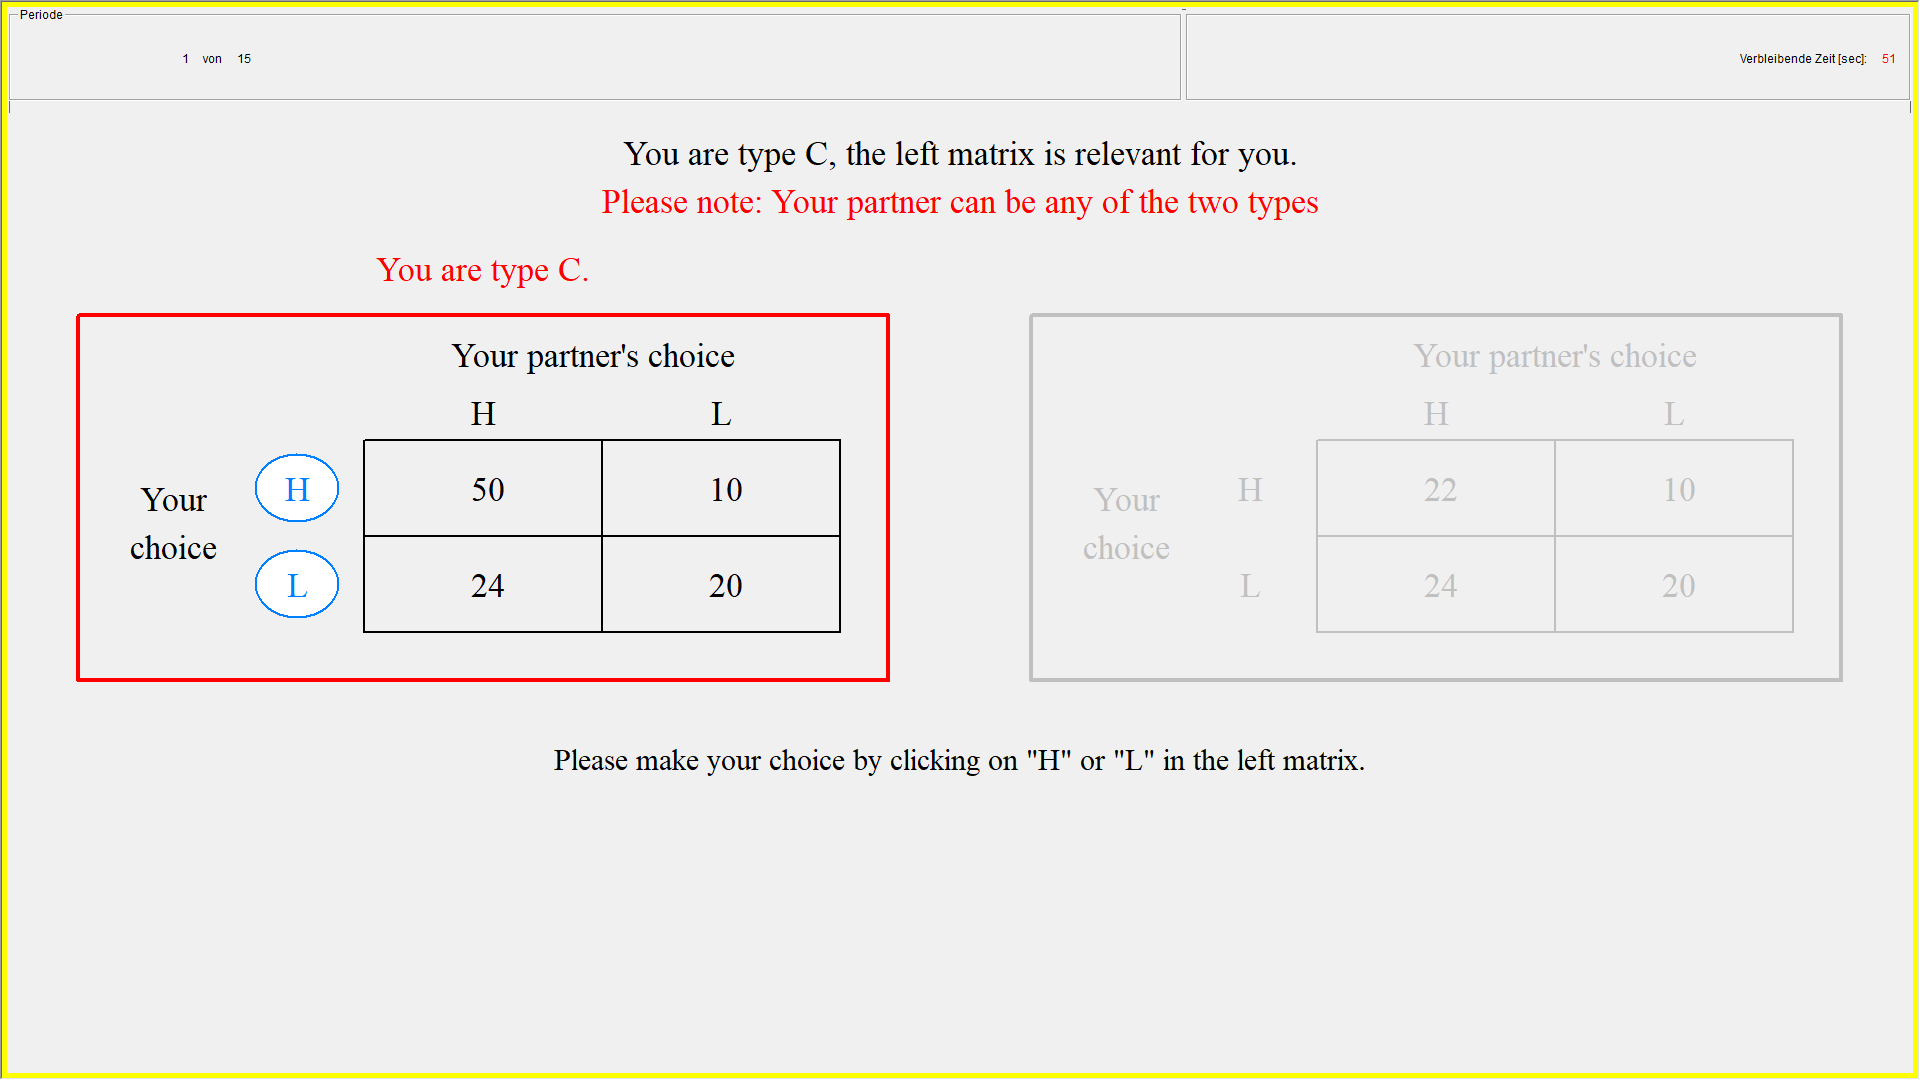
\includegraphics[width=1\textwidth]{fig1-NC-instructions.png}
  \label{fig:fig1-NC-instructions}
\end{figure}




You do not receive any information about the type of your partner, and your partner does not receive any information about your type. 

After your type and that of your partner have been randomly determined, you have to choose between two options, ``H'' and ``L", by clicking on the relevant blue button. When you are sure which choice to make, click on the blue button ``Confirm''.

 \begin{figure}[h]
   \centering
     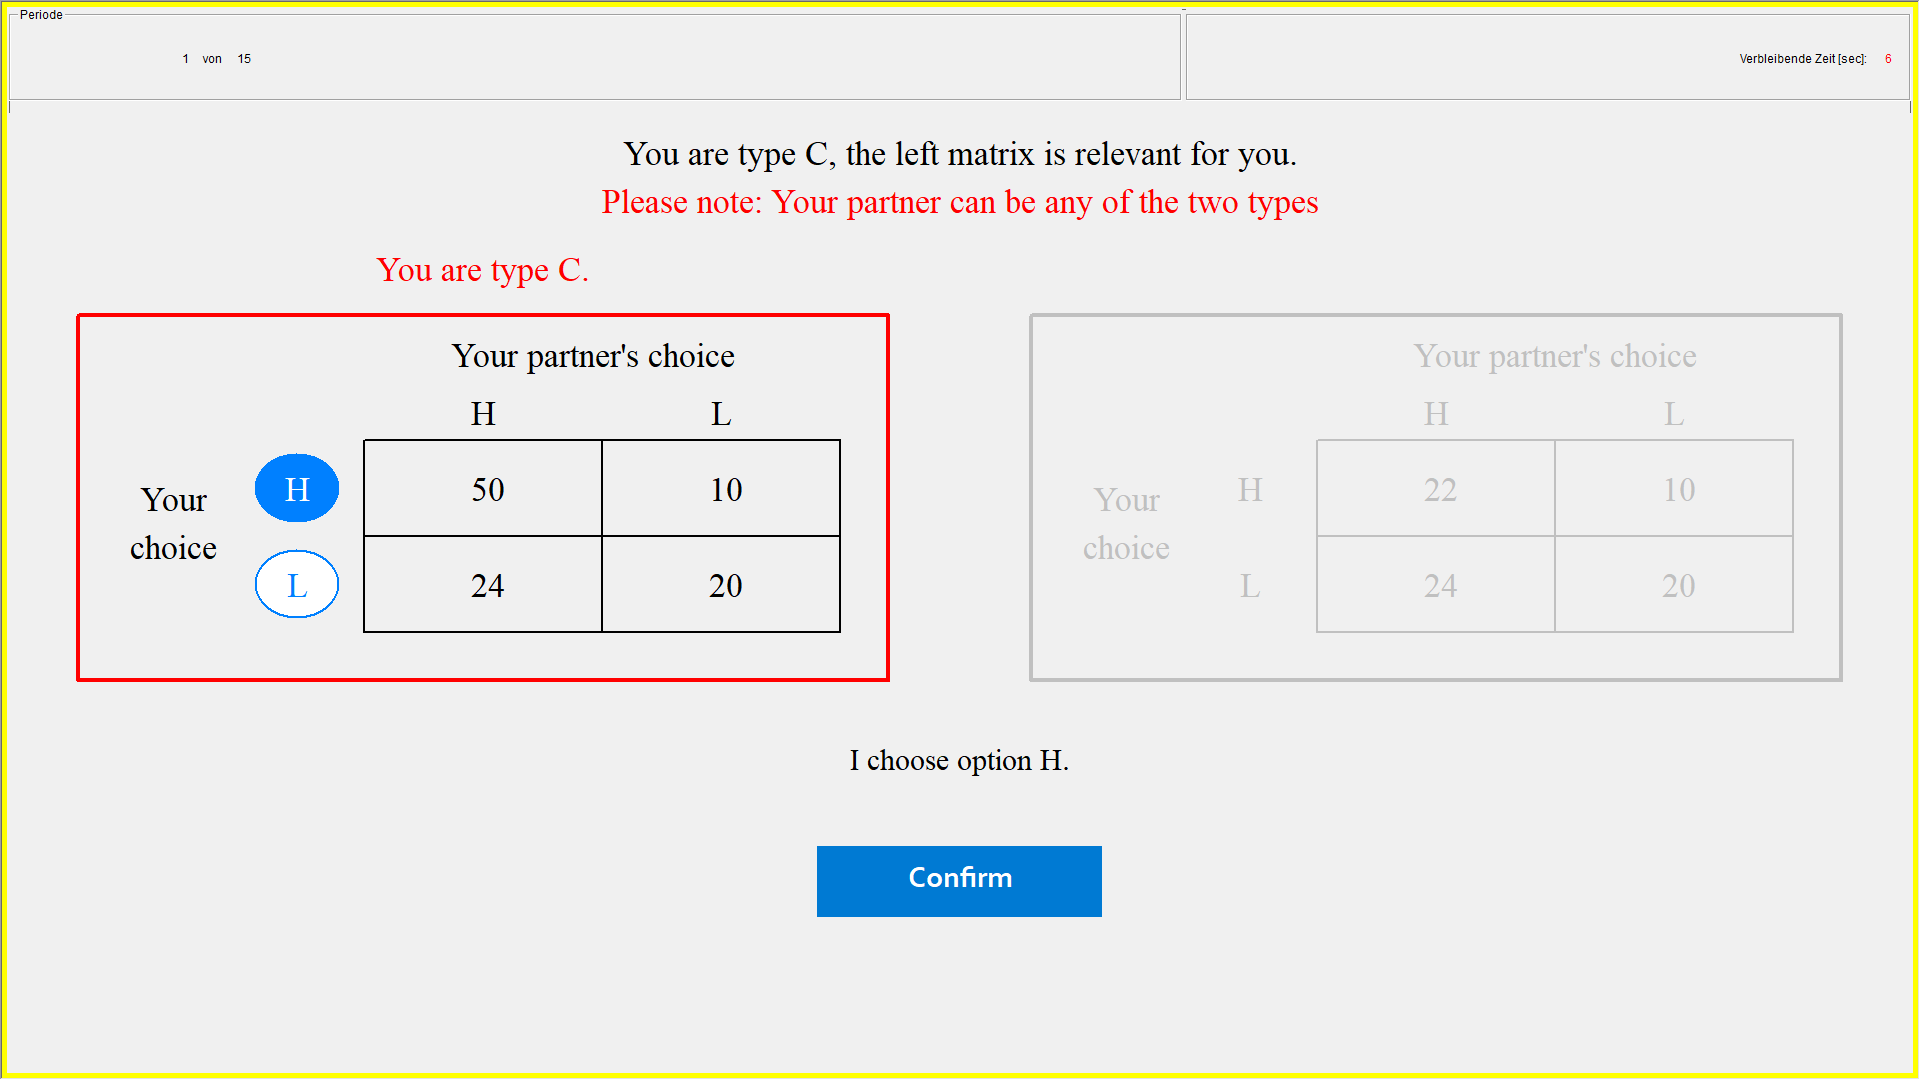
\includegraphics[width=.9\textwidth]{fig2-NC-instructions.png}
   \label{fig:fig2-NC-instructions}
 \end{figure}
 



You have at most one minute to decide which option to choose.

While you make your choice, your partner must also choose between ``H'' and ``L". You make your choice without knowing what your partner chooses, and your partner makes her/his choice without knowing your choice. 

After your decision and that of your partner the round ends, and your earnings for this round are calculated. As you can see from the screen-shot, your earning depends on your type, on your choice, and the choice of your partner. 

\textbf{Example}: You are of Type C, and therefore the left matrix is relevant for you. You choose H, and you partner chooses L. Therefore, your earnings are 10 ECUs in that round. Assume that your partner is of Type D in this round, i.e. the right matrix is relevant for her/him. In this case her/his earnings are 24. 

After the experiment ends, you will be asked to fill in a short questionnaire. After that you will be paid in private. Your overall earnings are the sum of the earnings you got in all 15 rounds. As already mentioned, the exchange rate between ECU and Euro is 25 ECU = 1 Euro. On top you will also get 4 Euros as a show up fee. The overall amount will appear on your screen, and paid to you in private by the experimenters. 

Do you have any questions? 




\textbf{Control Questionnaire}

The following questionnaire is anonymous and serves the sole purpose of verifying your understanding of this experiment. If you are uncertain about how to answer a questions, please consult the instructions or ask one of the experimenters.

Once you have finished the questionnaire, please raise your hand and an experimenter will come and check your answers.

1) You are of type D and you choose action L. Your partner is of type D and chooses action L.

What are your earnings in this round?
What are your partner’s earnings in this round?

2) You are of type C and choose action H. You partner is also of type C and chooses action H.

What are your earnings in this round?
What are your partner’s earnings in this round?


3) You are of type D and choose H. Your partner is of type C and chooses L.

What are your earnings in this round?
What are your partner’s earnings in this round?


\subsection{Instructions for the CT environment}

Welcome to the experiment on interactive decision-making, conducted by researchers from the Université libre de Bruxelles.

During this experiment you will earn an amount of money determined by your choices and by those of the other participants. All results will be analyzed anonymously, and your privacy is guaranteed. It is very important that you do not communicate with the other participants, neither verbally nor in any other way. If you have any question, please raise your hand and an experimenter will answer your question. If you communicate with the other participants during the experiment, you would have to leave the experiment without being paid. 

During the experiment your earnings are counted in Experimental Currency Units (ECUs). At the end of the experiment your earnings will be exchanged into Euros with an exchange rate of 1 Euro for 25 ECUs. You will be paid in cash immediately after the experiment. You will be paid privately, i.e. the other participants will not be informed about your earnings.

The whole experiment consists of 15 rounds. In each round you will be matched with a second participant, your ``partner". Your partner changes from round to round with your partner being determined randomly. It is possible that you might have the same partner during some rounds. But no participant gets any information about the identity of her/his partner. Therefore, it is impossible to identify the partner, and it is impossible to be identified by the partner.

Each round consists of 2 stages:

Stage 1: Your type and the type of your partner are determined. After being informed about your type (but not about the type of your partner), you decide whether you send a message to your partner or not. At the same time, your partner decides whether to send the a message to you or not.

Stage 2: You have to choose between two options, “H” or “L”. At the same time, your partner chooses between H and L. 

How much you earn in a certain round (your ``earnings") depends on your type, which option you choose, and which option your partner chooses. 

Detailed description of the two stages: 

\textbf{Stage 1}: At the beginning of each round your type is determined. You can be of two different types: Type “C” or Type “D”. If you are of Type C (as depicted on the screen-shot), the left earning matrix is relevant for your payment. If you are of Type D, the right earning matrix is relevant for you. 

\begin{figure}[h]
  \centering
    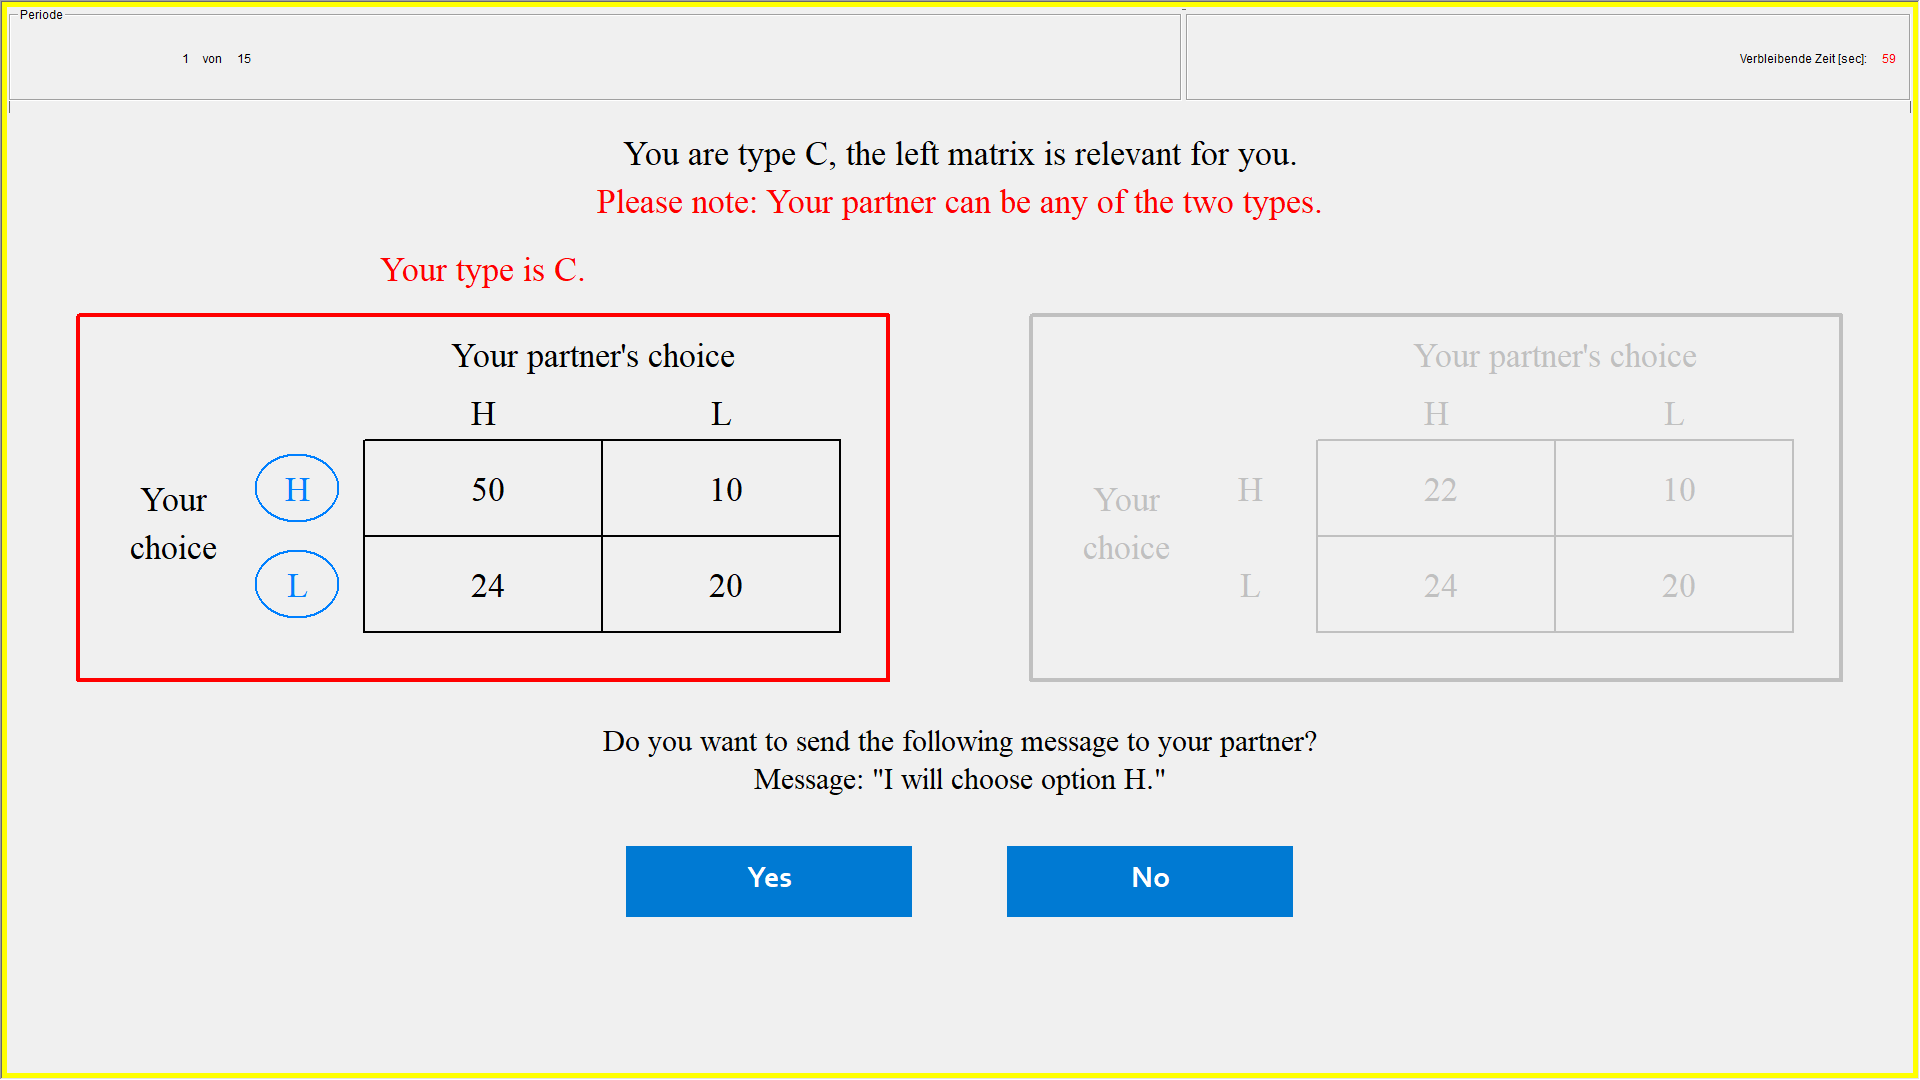
\includegraphics[width=.9\textwidth]{fig1-CT-instructions.png}
  \label{fig:fig1-CT-instructions}
\end{figure}


In every round your type will be determined randomly with equal probability (``fifty/fifty"). Similarly, the type of your partner is determined by the same random process. Your type and that of your partner might be the same, the types differ.
At the beginning of the round you will be informed about the type you are in this round. Your partner is also of the two possible types, but you will not be informed of which type he is. You only know that your partner is of Type C or Type D with equal probability.

Now you have to choose whether you want to send a message to your partner or not. The message refers to your choice in the Stage 2 and reads: “I will choose H” to your partner. If you want to send this message, click on the button ``Yes" on the screen below. If you do not want to send the message, click on the button ``No". 

You have at most one minute to decide whether you want to send the message or not. 

Note that the message is not binding for your actual choice in Stage 2 - if you send the message, you are nonetheless allowed to choose option ``L".

Your partner has to decide whether to send the same, non-binding message to you, too.

At the end of Stage 1, you get informed whether your partner sent you the message, and your partner gets informed whether you sent the message. 

\begin{figure}[h]
  \centering
    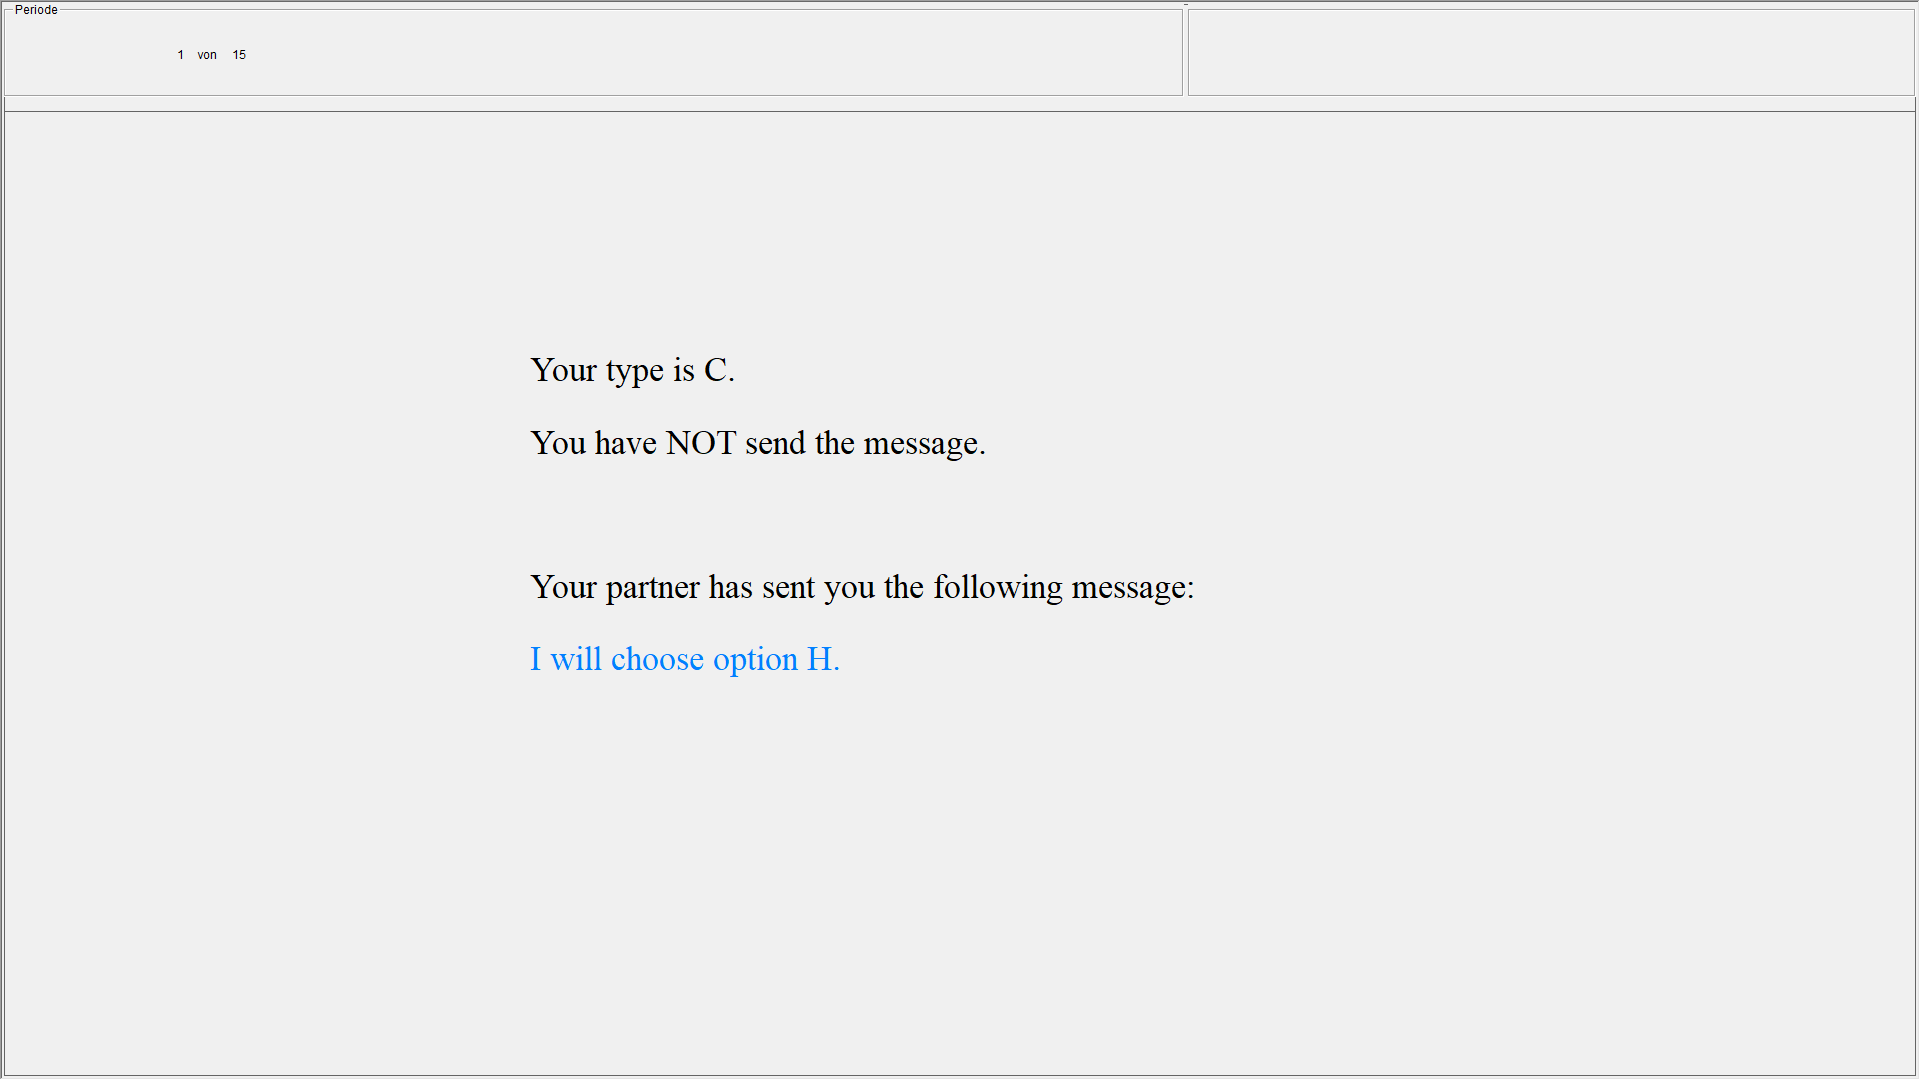
\includegraphics[width=.9\textwidth]{fig2-CT-instructions.png}
  \label{fig:fig2-CT-instructions}
\end{figure}


\textbf{Stage 2}: In stage 2 you have to choose between options, ``H'' and ``L", by clicking on the relevant blue button. 
If you are of Type C, the left matrix is relevant for you, if you are of type D, the right one.

When you are sure which choice to make, click on the blue button ``Confirm''.

\begin{figure}[h]
  \centering
    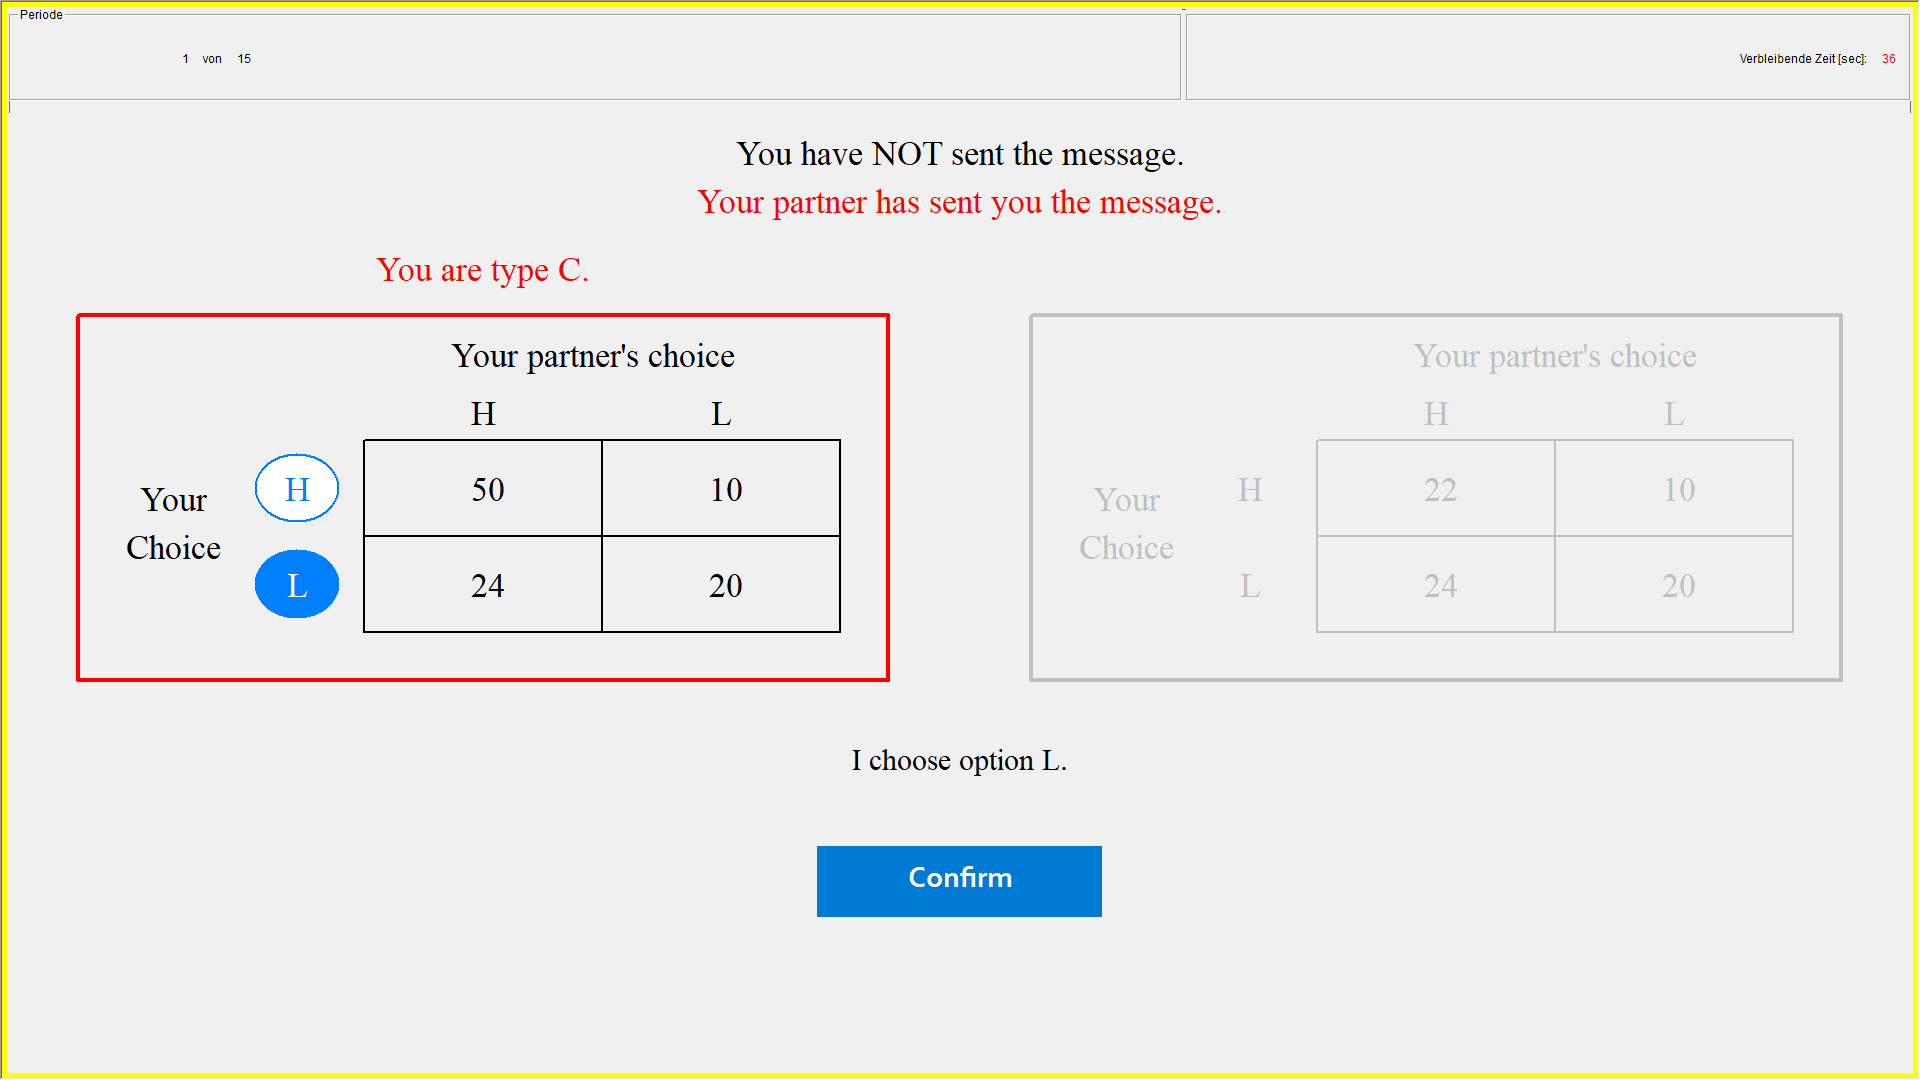
\includegraphics[width=.9\textwidth]{fig3-CT-instructions.png}
  \label{fig:fig3-CT-instructions}
\end{figure}

 
You have at most one minute to decide which option to choose.

While you make your choice, your partner must also choose between ``H'' and ``L". You make your choice without knowing what your partner chooses, and your partner makes her/his choice without knowing your choice. 

After the two stages the round ends, and your earnings for this round are calculated. As you can see from the screen-shot, your earning depends on your type, on your choice, and the choice of your partner. 

\textbf{Example}: You are of Type C, and therefore the left matrix is relevant for you. You choose H, and you partner chooses L. Therefore, your earnings are 10 ECUs in that round. Assume that your partner is of Type D in this round, i.e. the right matrix is relevant for her/him. In this case her/his earnings are 24. 

After the experiment ends, you will be asked to fill a short questionnaire. The sum of your earnings will be transformed into Euros with a change rate of 25 ECUs to 1 Euro. On top you will also get 4 Euros as a show up fee. The overall amount will appear on your screen, and paid to you in private by the experimenters. 

Do you have any questions? 

\textbf{Control Questionnaire}

Dear Participant,

the following questionnaire is anonymous and serves the sole purpose of verifying your understanding of this experiment. If you are uncertain about how to answer a questions, please consult the instructions or ask one of the experimenters.

Once you have finished the questionnaire, please raise your hand and an experimenter will come and check your answers.

1) You are of type D and you choose action L. Your partner is of type D and chooses action L.

What are your earnings in this round?
What are your partner’s earnings in this round?

2) You are of type C and choose action H. You partner is also of type C and chooses action H.

What are your earnings in this round?
What are your partner’s earnings in this round?


3) You are of type D and choose H. Your partner is of type C and chooses L.

What are your earnings in this round?
What are your partner’s earnings in this round?


\subsection{Instructions for the FC environment}

Welcome to the experiment on interactive decision-making, conducted by researchers from the Université libre de Bruxelles.

During this experiment you will earn an amount of money determined by your choices and by those of the other participants. All results will be analyzed anonymously, and your privacy is guaranteed. It is very important that you do not communicate with the other participants, neither verbally nor in any other way. If you have any question, please raise your hand and an experimenter will answer your question. If you communicate with the other participants during the experiment, you would have to leave the experiment without being paid. 

During the experiment your earnings are counted in Experimental Currency Units (ECUs). At the end of the experiment your earnings will be exchanged into Euros with an exchange rate of 1 Euro for 25 ECUs. You will be paid in cash immediately after the experiment. You will be paid privately, i.e. the other participants will not be informed about your earnings.

The whole experiment consists of 15 rounds. In each round you will be matched with a second participant, your ``partner". Your partner changes from round to round with your partner being determined randomly. It is possible that you might have the same partner during some rounds. But no participant gets any information about the identity of her/his partner. Therefore, it is impossible to identify the partner, and it is impossible to be identified by the partner.

Each round consists of 2 stages:

Stage 1: Your type and the type of your partner are determined. After being informed about your type (but not about the type of your partner), you decide whether you send a message to your partner or not. At the same time, your partner decides whether to send the a message to you or not.

Stage 2: You have to choose between two options, “H” or “L”. At the same time, your partner chooses between H and L. 

How much you earn in a certain round (your ``net-earnings") depends on your type, whether you send a message to your partner or not, which option you choose, and which option your partner chooses. 

Detailed description of the two stages: 

\textbf{Stage 1}: At the beginning of each round your type is determined. You can be of two different types: Type “C” or Type “D”. If you are of type C (as depicted on the screen-shot), the left earning matrix is relevant for your payment. If you are of Type D, the right earning matrix is relevant for you. 
 
\begin{figure}[h]
  \centering
    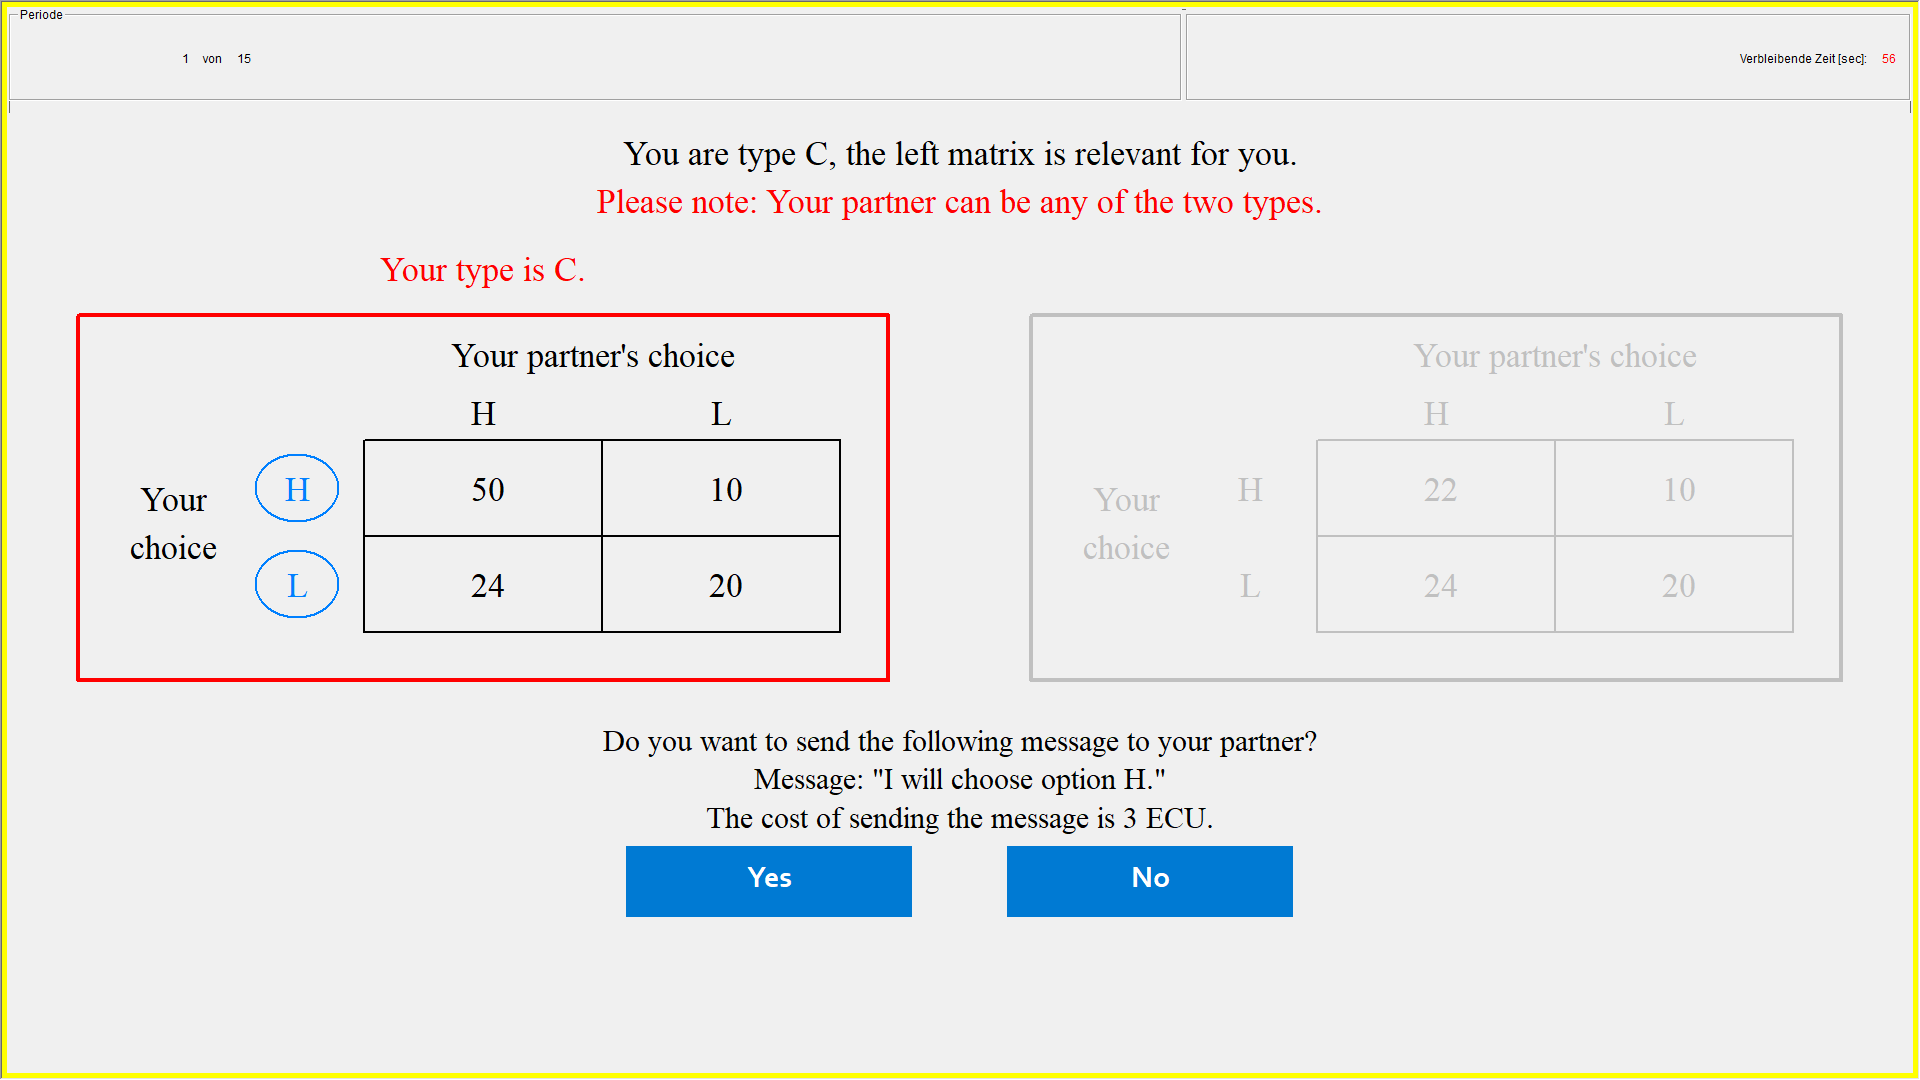
\includegraphics[width=.9\textwidth]{fig1-FC-instructions.png}
 \label{fig:fig1-FC-instructions}
\end{figure}

In every round your type will be determined randomly with equal probability (``fifty/fifty"). Similarly, the type of your partner is determined by the same random process. Your type and that of your partner might be the same, or the types differ.

At the beginning of the round you will be informed about the type you are in this round. Your partner is also of the two possible types, but you will not be informed of which type he is. You only know that your partner is of Type C or Type D with equal probability.

Now you have to choose whether you want to send a message to your partner or not. The message refers to your choice in the Stage 2 and reads: “I will choose H” to your partner. If you want to send this message, click on the button ``Yes'' on the screen below. If you do not want to send the message, click on the button ``No''. 

Sending the message costs you 3 ECUs, while sending no message costs you nothing.

You have at most one minute to decide whether you want to send the message or not. 

Note that the message is not binding for your actual choice in Stage 2 - if you send the message, you are nonetheless allowed to choose option ``L''.

Your partner has to decide whether to send the same, non-binding message to you, too.

At the end of Stage 1, you get informed whether your partner sent you the message, and your partner gets informed whether you sent the message. 

\begin{figure}[h]
  \centering
    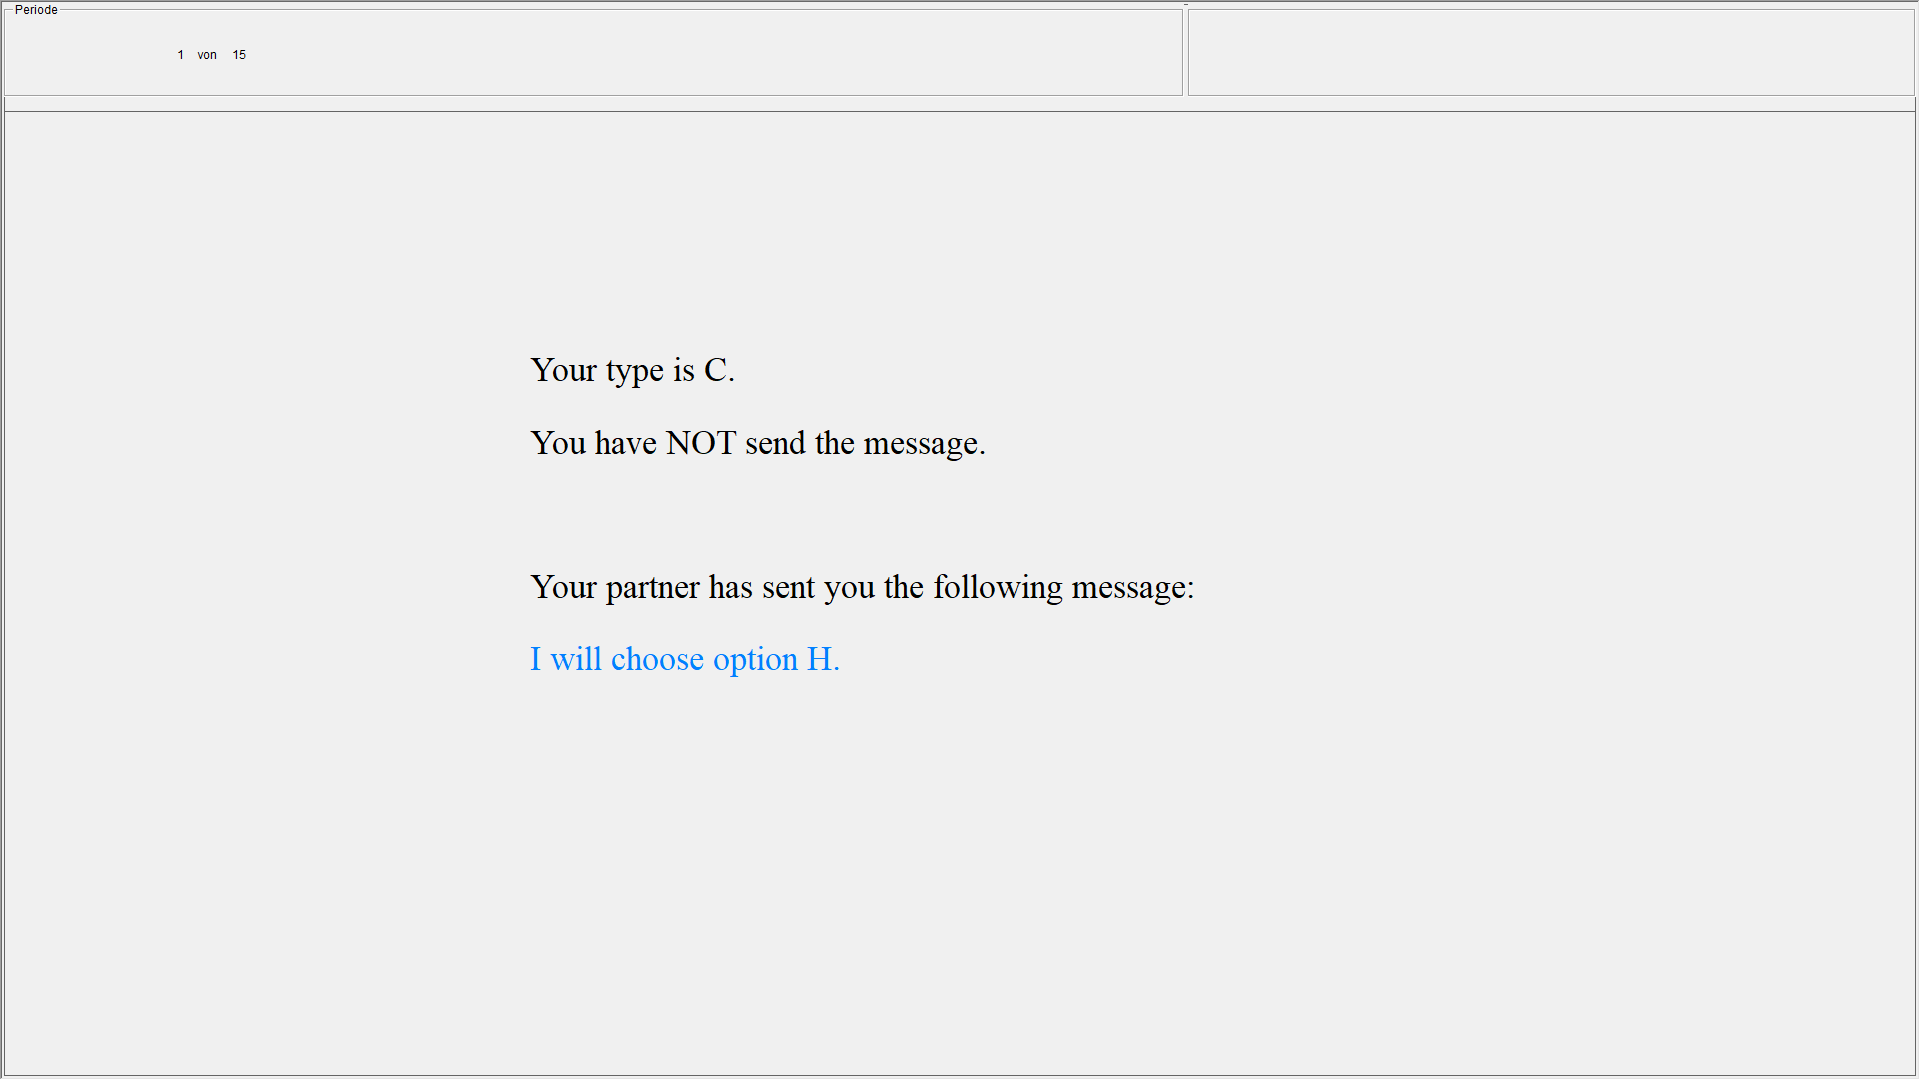
\includegraphics[width=.9\textwidth]{fig2-CT-instructions.png}
\label{fig:fig2-CT-instructions}
\end{figure}


\textbf{Stage 2}: In stage 2 you have to choose between options, ``H'' and ``L'', by clicking on the relevant blue button. 
If you are of Type C, the left matrix is relevant for you, if you are of type D, the right one.

When you are sure which choice to make, click on the blue button ``Confirm''.

 \begin{figure}[h]
   \centering
     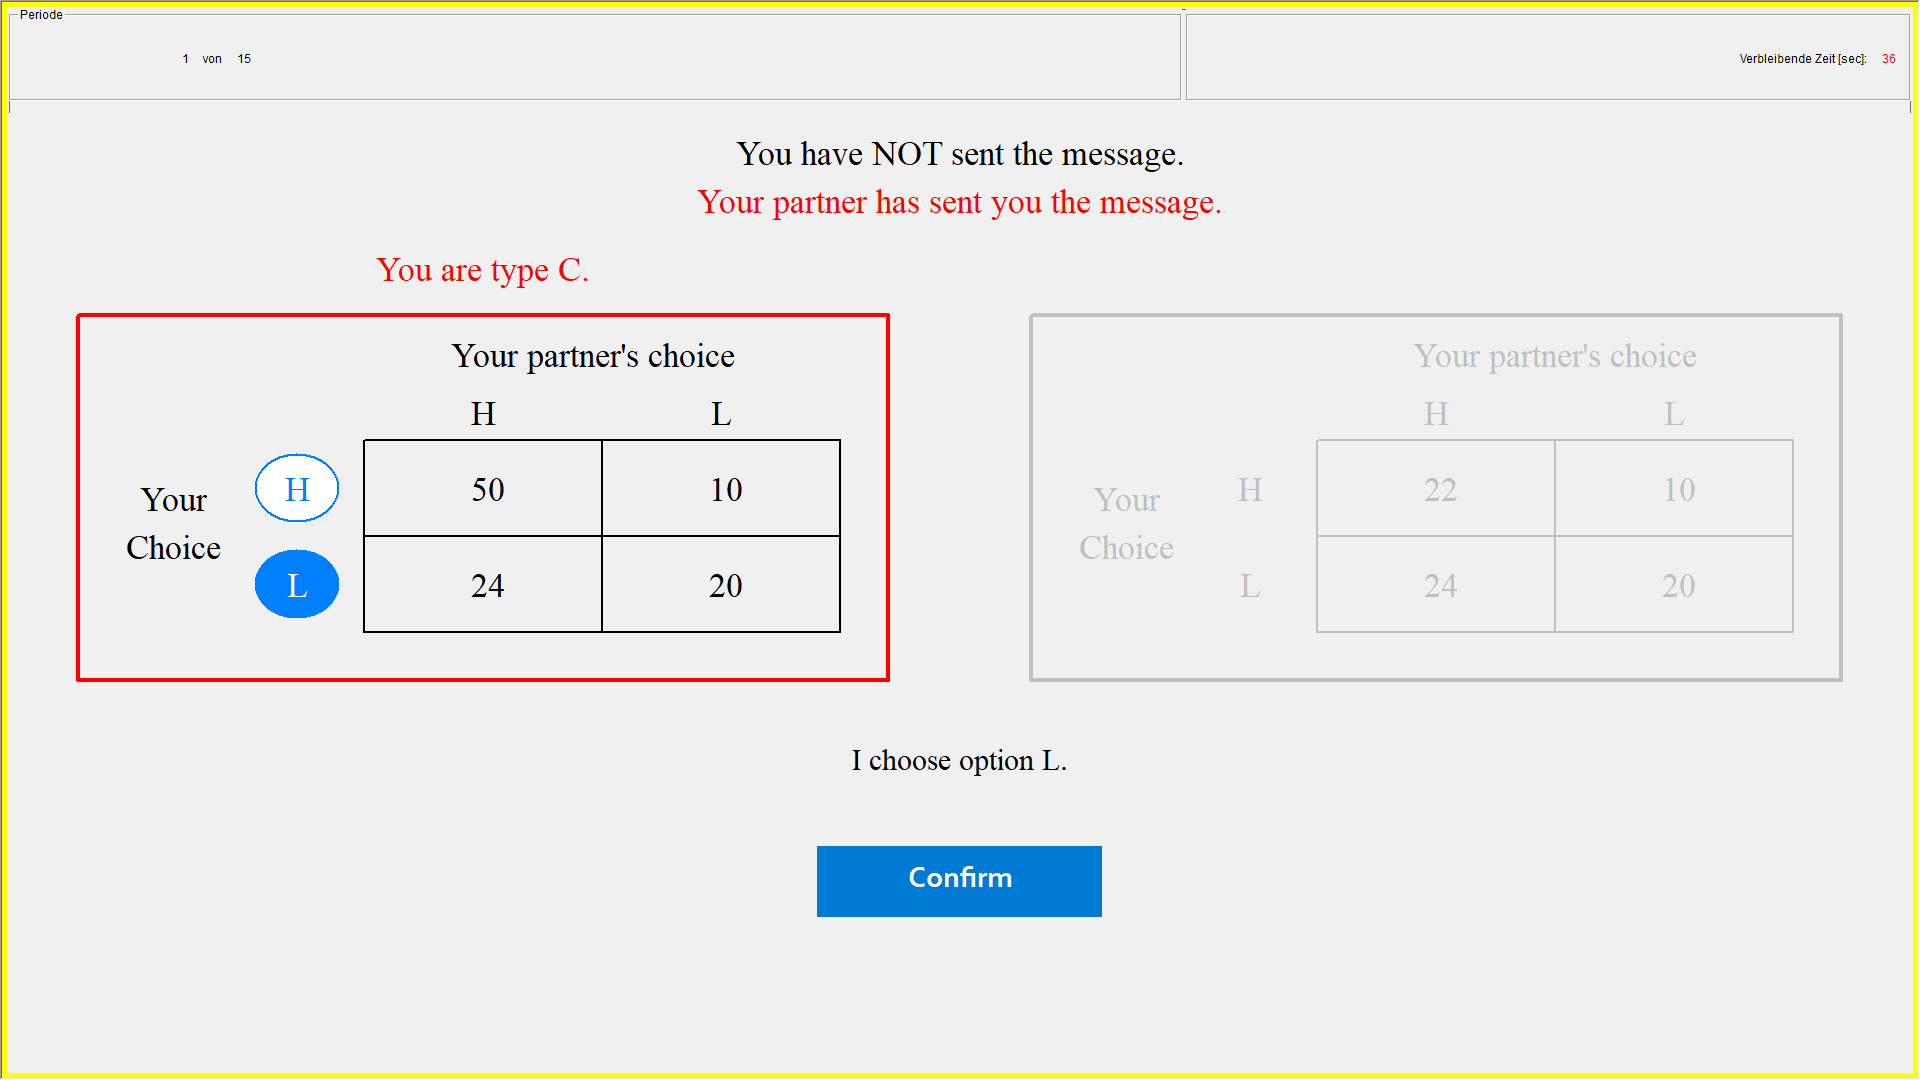
\includegraphics[width=.9\textwidth]{fig3-FC-instructions.png}
   \label{fig:fig3-FC-instructions}
 \end{figure}
 

You have at most one minute to decide.

While you make your choice, your partner must also choose between ``H'' and ``L". You make your choice without knowing what your partner chooses, and your partner makes her/his choice without knowing your choice. 

After the two stages the round ends, and your net-earnings for this round are calculated. As you can see from the screen-shot, your net-earnings depend on your type, whether you send a message to your partner or not, which option you choose, and which option your partner chooses. 

\textbf{Example}: You are of Type C, and therefore the left matrix is relevant for you. You send the message and this costs you three ECUs. You choose H, and you partner chooses L. Therefore, your earnings are 10-3= 7 ECUs in that round. Assume that your partner is of Type D in this round, i.e. the right matrix is relevant for her/him, and (s)he does not send a message. In this case her/his earnings are 24. 

After the experiment ends, you will be asked to fill a short questionnaire. The sum of your earnings will be transformed into Euros with a change rate of 25 ECUs to 1 Euro. On top you will also get 4 Euros as a show up fee. The overall amount will appear on your screen, and paid to you in private by the experimenters. 

Do you have any questions? 

\textbf{Control Questionnaire}

The following questionnaire is anonymous and serves the sole purpose of verifying your understanding of this experiment. If you are uncertain about how to answer a questions, please consult the instructions or ask one of the experimenters.

Once you have finished the questionnaire, please raise your hand and an experimenter will come and check your answers.

1) You are of type D, you send the message, and you choose action L. Your partner is of type 2, (s)he does not send the message, and chooses action L.

What are your earnings in this round?
What are your partner’s earnings in this round?

2) You are of type C, you do not send the message, and you choose action H. Your partner is of type C, (s)he sends the message, and chooses action H.

What are your earnings in this round?
What are your partner’s earnings in this round?


3) You are of type D, you do not send the message, and you choose action H. Your partner is of type C, (s)he does not send the message, and chooses action L.

What are your earnings in this round?
What are your partner’s earnings in this round?








\bibliographystyle{agsm}
\bibliography{collusion}
\end{document}